\newcommand{\pluseq}{\mathrel{+}=}

% make bold shape available for listings
\renewcommand{\ttdefault}{pcr}
\lstset{language=[90]Fortran,
  basicstyle=\ttfamily\lst@ifdisplaystyle\scriptsize\fi,
  keywordstyle=\bfseries,
  comment=[l]{!\ },
  escapechar=@,
%  numbers=left,
  tabsize=4,
}


\chapter{Efficiency of High Order Spectral Element Methods on Petascale Architectures}

\makeatletter
\newcommand{\chapterauthor}[1]{%
  {\parindent0pt\vspace*{-25pt}%
  \linespread{1.1}\large\scshape#1%
  \par\nobreak\vspace*{35pt}}
  \@afterheading%
}
\makeatother

\vspace{20pt}

\chapterauthor{Maxwell Hutchinson, Alexander Heinecke, Hans Pabst, Greg Henry, Matteo Parsani, and David Keyes}

% a short form should be given in case it is too long for the running head
%\titlerunning{Lecture Notes in Computer Science: Authors' Instructions}

% the name(s) of the author(s) follow(s) next
%
% NB: Chinese authors should write their first names(s) in front of
% their surnames. This ensures that the names appear correctly in
% the running heads and the author index.
%
%\author{Maxwell Hutchinson\inst{1} \and Alexander Heinecke\inst{2}  \and Hans Pabst\inst{3}  
%\and Greg Henry\inst{4}
%\and Matteo Parsani\inst{5}
%\and David Keyes\inst{5}
%}

%\institute{
%Department of Physics, University of Chicago, 5720 S. Ellis Ave, Chicago IL, 60637, USA
%Department of Physics, University of Chicago, Chicago IL, USA
%\and
%Intel Corporation, 2200 Mission College Blvd., Santa Clara CA, 95054, USA
%Intel Corporation, Santa Clara CA, USA
%\and
%Intel Semiconductor AG, Badenerstrasse 549, 8048 Zurich, Switzerland
%Intel Semiconductor AG, Zurich, Switzerland
%\and
%Intel Corporation, 2111 NE 25th Avenue, Hillsboro OR, 97124, USA
%Intel Corporation, Hillsboro OR, USA
%\and
%Extreme Computing Research Center, KAUST, Thuwal, 23955, KSA
%}


%\maketitle


\section{Abstract}
High order methods for the solution of PDEs expose a trade-off between computational cost and accuracy on a per degree of freedom basis.
In many cases, the cost increases due to higher arithmetic intensity while affecting data movement minimally.
As architectures tend towards wider vector instructions and expect higher arithmetic intensities, the best order for a particular simulation may change.

This study highlights preferred orders by identifying the high order efficiency frontier of the spectral element method implemented in Nek5000 and NekBox: the set of orders and meshes that minimize computational cost at fixed accuracy.
First, we extract Nek's order-dependent computational kernels and demonstrate exceptional hardware utilization by hardware-aware implementations.
Then, we perform production-scale calculations of the nonlinear single mode Rayleigh-Taylor instability on BlueGene/Q and Cray XC40-based supercomputers to highlight the influence of the architecture.
Accuracy is defined with respect to physical observables, and computational costs are measured by the core-hour charge of the entire application.
The total number of grid points needed to achieve a given accuracy is reduced by increasing the polynomial order.
On the XC40 and BlueGene/Q, polynomial orders as high as 31 and 15 come at no marginal cost per timestep, respectively.
Taken together, these observations lead to a strong preference for high order discretizations that use fewer degrees of freedom.
From a performance point of view, we demonstrate up to 60\% full application bandwidth utilization at scale and achieve $\approx$ 1 PFlop/s of compute performance in Nek's most flop-intense methods.

\section{Introduction}
\label{sec:introduction}
The solution of partial differential equations (PDEs) is a core problem in HPC, with particular application to computational materials science and fluid dynamics.
PDEs are solved by discrete approximation: space and time are sampled and the PDEs is translated into a relation on those samples.
From a mathematical point of view, these approximations are characterized by stability conditions and convergence rates.
Schemes which do not satisfy stability conditions usually fail catastrophically with values that diverge to infinity.
The convergence rate describes the relationship between the resolution and the error.
For a characteristic inter-sample spacing $h$, a method is of order $p$ if the error goes as $h^p$.
High order methods are schemes with convergence rates higher than third order~\cite{wang2013high}, many of which expose the order as a user input.

From a computational point of view, the approximations are characterized by sparsity, locality, and arithmetic intensity.
As the order increases, the sparsity and locality typically decrease while the arithmetic intensity increases.
The improved convergence rates are `paid for' with more floating point operations (FLOP), on a per sample basis, while, for a given error tolerance, the number of samples can be decreased.
The relationship between these computational characteristics and computational cost is complicated by features common to modern architectures: vector instructions, deep caches, and arithmetic-to-data movement imbalance.

Here, we explore the relationship between order, accuracy, cost, and architecture.
We identify the user-facing properties of high order methods: the accuracy in observables, time to solution, resource usage, and required scale.
We also identify the user-defined inputs: the physical problem, the order, the total number of samples, the number of processors, and the computer architectures.
To make the study more practical, we focus on the specific task of optimizing a study of the single-mode Rayleigh-Taylor instability (smRTI) as a parameter sweep over Grashof and Prandtl numbers.
This is a high throughput use-case, where the relevant cost is resource usage and scale is fixed with respect to the size of the problem and assumed to not be a limitation.
This leaves us with the accuracy and resource usage versus the order, number of samples, and computer architectures.

We select the NekBox version of the Nek5000 code (together: Nek), which
implements the spectral element method (SEM)~\cite{patera1984spectral} with tunable order, is known to scale to a million ranks~\cite{nekscaling}, and has been used for Rayleigh-Taylor problems in the past~\cite{hutchinson2015direct}.
NekBox takes advantage of static, uniform meshes to solve the coarse part of the preconditioner with FFTs or DCTs, improving efficiency and scalability.
We extract representative order-dependent kernels from Nek and analyze their
performance on BlueGene/Q and Cray XC40 supercomputers.

We also conduct a set of application benchmarks to measure the cost and accuracy.
The cost is computed in core-hours, in the same way most users are charged.
The accuracy is computed with respect to the smRTI's bubble height and mix volume, which are the most common observables studied in the smRTI community.
The benchmarks vary the order and total number of samples, and are conducted on the Mira and Shaheen XC40 supercomputers at Argonne Leadership Computing Facility (ALCF) and KAUST Supercomputing Laboratory (KSL), respectively.


\subsection{Outline}
In \sref{math}, we review the SEM as implemented in Nek.
In \sref{implementation}, we introduce LIBXSMM for hardware-aware implementation of Nek's performance critical kernels, and demonstrate their performance in isolation.
In \sref{benchmarks}, we perform a convergence/performance study of SEM discretizations for the smRTI problem and present full-application performance at scale.
\sref{conclusion} concludes with a discussion of preferred orders on the BlueGene/Q and Cray XC40 supercomputers. 



\section{Nek's Computational Core}
\label{sec:math}
\subsection{Governing equations and time-splitting}
Nek5000 and NekBox solve the incompressible Navier--Stokes equations:
\begin{equation}
\frac{\partial u}{\partial t} + u \cdot \nabla u = - \frac{1}{\rho} \nabla p + \nu \nabla^2 u + f \qquad
\nabla \cdot u = 0,
\end{equation}
where $u$ is the flow velocity, 
$\rho$ is the fluid density,
$p$ is the pressure,
$\nu$ is the kinematic viscosity,
and $f$ consists of user-defined forcing terms.
Additionally, Nek can solve advection-diffusion equations for scalars, such as the temperature or mass fraction:
\begin{equation}
\frac{\partial \phi_i}{\partial t} + u \cdot \nabla \phi_i =  \alpha_i \nabla^2 \phi_i + q_i,
\end{equation}
where $\phi_i$ is the scalar value, 
$\alpha_i$ is the diffusivity,
and $q_i$ is a user-defined source term, each for the $i$th scalar.

The time derivative is discretized with a backward difference formula (BDF), within which the nonlinear and forcing terms are extrapolated (EX):
\begin{equation}\elabel{semi}
\sum_{j=0}^k \frac{\beta_i}{\Delta t} M u_i^{n-j} = - \frac{1}{\rho} D_i p^n + \nu K u_i^n + \sum_{j=1}^n a_j\left[M f_i^{n-j} - (C u_i)^{n-j} \right],
\end{equation}
where $M$ is the mass matrix,
$C$ is the convection matrix,
$K$ is the stiffness matrix,
$D$ is the gradient matrix,
$i \in \{1,2,3\}$ are the spatial dimension indexes, 
$n$ is the time level index, and
$k$ is the formal order of accuracy of the BDF/EX scheme.
The pressure is decoupled from the new velocity, $u^n$, by taking the divergence:
\begin{equation} \elabel{pres}
K p^n = D_i \sum_{j=1}^n a_j F_i^{n-j},
\end{equation}
where $F_i^n = M f_i^n - (C u_i)^n$,
which results in the Poisson pressure equation.
Finally, the pressure is incorporated back into \eref{semi}:
\begin{equation} \elabel{vel}
\left[\nu K + \frac{b_0}{\Delta t} M \right] u_i^n = -D_i \frac{p^n}{\rho} + \sum_{j=1}^k \left[a_j F_i^{n-j} + \frac{b_j}{\Delta t} M u^{n-j} \right], 
\end{equation}
which results in three Helmholtz velocity equations.

\begin{comment}
The semi-discrete incompressible Navier--Stokes equations can be written as~\cite{Deville2002}:
\begin{equation} \label{eqn:NS1}
M \frac{d u_i^{n+1}}{dt} + \text{Re}~ C u_i^{n+1} + K u_i^{n+1} - D_i^T p^{n+1} =  M f_i^{n+1} \qquad \sum_i -D_i u_i^{n+1} = 0,
\end{equation}
where $M$ is the mass matrix,
$C$ is the convection matrix,
$K$ is the stiffness matrix,
$D$ is the gradient matrix,
$i \in \{1,2,3\}$ indexes spatial dimensions, and
$n$ indexes time.
The temporal derivative is expressed with the third-order backwards difference formula, and the convection operator with third-order explicit Adams-Bashforth extrapolation~\cite{Deville2002}.
The advection-diffusion equations are treated similarly, but without a pressure term, and solved first.
The forcing terms in this study depend only on $\phi$, and are evaluated directly at the next time level ($t^{n+1}$)~\cite{Tomboulides1997}.
\end{comment}

\begin{comment}
\begin{equation} \elabel{bdf}
\left(\frac{11}{6 \Delta t} M + K\right) u^{n+1}_i - D^T_i p^{n+1} = \frac{M}{\Delta t} \left(3 u^n_i - \frac{3}{2} u^{n-1}_i + \frac{1}{3} u^{n-2}_i \right) + M f_i^{n+1} - \text{Re} C u^{n+1}_i 
\end{equation}
The convection matrix and external force are extrapolated to third-order:
\begin{equation}
C u_i^{n+1} \approx \left(3 C u_i^n - 3 C u_i^{n-1} + C u_i^{n-2}\right)
\end{equation}
\end{comment}

\begin{comment}
If we group the explicit terms together as $F_i^{n+1}$ and define the Helmholtz operator $H_i = (11/6\Delta t)M + K$, 
we can re-write the governing equations in matrix form:
\begin{equation} \label{eqn:stokes}
\begin{pmatrix} \mathbf{H} & -\mathbf{D}^T \\ -\mathbf{D} & 0 \end{pmatrix} \begin{pmatrix} v^{n+1} \\ p^{n+1} \end{pmatrix} = \begin{pmatrix} \mathbf{F} \\ 0 \end{pmatrix},
\end{equation}
where $\mathbf{D} = \left[ D_1, D_2, D_3 \right]$ is the divergence matrix,
and $\mathbf{A} = \text{diag}(A_1, A_2, A_3)$ otherwise.
This expression is factored by approximating $\mathbf{H}^{-1} \approx (6 \Delta t)/11 \mathbf{M}^{-1}$:
\begin{equation} \label{eqn:NS2}
\begin{pmatrix} I & 0 \\  \frac{6 \Delta t}{11} \mathbf{D} \mathbf{M}^{-1} & I \end{pmatrix} \begin{pmatrix} \mathbf{H} & \quad-\frac{6 \Delta t}{11} \mathbf{H} \mathbf{M}^{-1} \mathbf{D}^T \\ 0 & \quad\frac{6 \Delta t}{11} \mathbf{D} \mathbf{M}^{-1} \mathbf{D}^T \end{pmatrix} \begin{pmatrix} v^{n+1} \\ p^{n+1} \end{pmatrix} \approx \begin{pmatrix} \mathbf{F} \\ 0 \end{pmatrix}.
\end{equation}
Introducing a compressible intermediate velocity $\hat{v}$, and its divergence:
\begin{equation} \label{eqn:NS3}
\begin{pmatrix} I & 0 \\ \frac{6 \Delta t}{11} \mathbf{D} \mathbf{M}^{-1} & I \end{pmatrix}  \begin{pmatrix} \hat{v} \\ \nabla \cdot \hat{v} \end{pmatrix} = \begin{pmatrix} \mathbf{F} \\ 0 \end{pmatrix} \qquad 
\begin{pmatrix} \mathbf{H} & -\frac{6 \Delta t}{11} \mathbf{H} \mathbf{M}^{-1} \mathbf{D}^T \\ 0 & \frac{6 \Delta t}{11} \mathbf{D} \mathbf{M}^{-1} \mathbf{D}^T \end{pmatrix} \begin{pmatrix} v^{n+1} \\ p^{n+1} \end{pmatrix} \approx \begin{pmatrix} \hat{v} \\ \nabla \cdot \hat{v} \end{pmatrix}.
\end{equation}

The scheme in \eref{NS3} represents a sequence of solves:
\begin{inparaenum}[\itshape a\upshape)]
\item explicit convection $\hat{v} = F$;
\item Poisson pressure equation $\bigtriangleup p^{n+1} = \nabla \cdot \hat{v}$; and
\item Helmholtz velocity equation $H v_i^{n+1} = \hat{v}_i - \nabla_i p^{n+1}$.
\end{inparaenum}
\end{comment}

These steps are the core of Nek5000 and NekBox: the explicit calculation of
right-hand sides, a Poisson solver for the pressure, \eref{pres}, and a Helmholtz solver for the three components of the velocity, \eref{vel}.

\subsection{Spectral element method}
Nek5000 and NekBox implement SEM: a two-level discretization constructed from tensor products of Gauss-Lobatto-Legendre (GLL) quadrature points within elements and continuity across elements, forming a mesh.
Fields are represented as
\begin{equation}
u(x,y,z) = \sum_{i=0}^p \sum_{j=0}^p \sum_{k=0}^p \tilde{u}_{i,j,k,e} h_i(x) h_j(y) h_k(z), 
\end{equation}
where $p$ is the polynomial order of the method,
$e(x,y,z)$ is the index of the element in the mesh,
and $h_i(x)$ is the $i$th Lagrange polynomial through the GLL points of element $e$.
The choice of Lagrange polynomials leads to diagonal mass matrices and related geometric factors.
The spectral basis within each element enjoys exponential convergence with respect to the polynomial order.
GLL points do not sample space uniformly, so concatenating elements is more effective at reducing grid spacing than increasing spectral order.
Many small elements are also better able to match complex geometries than fewer larger ones.
The spectral element method is able to satisfy both the demand for geometric flexibility with quasi-uniform coverage and spectral convergence, but the particular choice of the spectral order versus the number of elements can be difficult to optimize.

In SEM, operators are written as the product of a local operator and \textit{direct stiffness summation}, which enforces continuity at the shared element boundaries.
The local operators are decomposed into tensor products of 1D operators.
The general form of an operator $A$ is:
\begin{equation}
A = (A_x \times I_y \times I_z) + (I_x \times A_y \times I_z) + (I_x \times I_y \times A_z),
\end{equation}
where $A_x, A_y, A_z$ are 1D projections of the operator $A$ and $I$ is the
identity matrix.
In this way, linear operators from $R^{N \times N \times N} \rightarrow R^{N \times N \times N}$ can be evaluated in $O(N^4)$ operations instead of $O(N^6)$~\cite{tufo1999terascale}.
This reduces the arithmetic intensity of operator evaluation in SEM to $O(p)$.

\subsection{Computational profile}
The spectral element method, as implemented in Nek5000 and NekBox, spends its time in three computational motifs: sparse communication, vector-vector, and matrix-matrix.
The sparse communication comes from the direct stiffness summations and the coarse part of the pressure preconditioner.
The vector-vector workload comes from inner products in the solvers and frequent rescaling by geometric factors, which are shaped like the diagonal mass matrix.
The matrix-matrix workload comes from local operator evaluation.

The direct-stiffness summation is handled by a stand-alone library~\cite{ivanov2015evaluation,otten2016}. 
In Nek, the pressure solve takes roughly 30\% of the run-time, distributed between operator application, inner products, and the preconditioner.
The preconditioner is multigrid with a local additive Schwarz part and the global coarse part~\cite{lottes2005hybrid}.
In NekBox, the coarse part of the pressure preconditioner is solved directly with FFTs or fast cosine transforms, and typically takes less than 5\% of the total runtime.
Local communication makes up a small portion of NekBox's run time at moderate numbers of points per processor, and Nek5000 and NekBox weak scale effectively to millions of ranks~\cite{hutchinson2015direct}.

The efficiency of the vector-vector computation is generally left to the compiler, aided by aggressive loop merging in the solvers.
For architectures that support them, the compiler needs help issuing non-temporal stores, which are performance optimal only if the working set is larger than the last level cache.
These stores are used in parts of the solver and local element evaluation, and are discussed further in \sref{implementation}.

Matrix-matrix is the most accessible and performance critical portion of the workload.
In particular, it is the only part of Nek that depends on the order, holding the
total degrees of freedom (DOFs) fixed.

\subsection{Order-dependent kernels}
\label{sec:operators}
There are two matrix-matrix routines that sit inside of the iterative solvers: the Helmholtz operator and a basis transformation.

The Helmholtz operator is found on the left-hand side of \eref{pres} and \eref{vel}:
$$ H u = (h_1 K + h_2 M) u, $$
where the special case of $h_2 = 0$ is the Poisson operator.
\begin{algorithmic}[1] \small
\Procedure{Local Helmholtz operator}{$Hu, u, h_1, h_2$}
\State $(H u)_{i,j,k} \gets (G_x)_{i,j,k} * \sum_l (K_x)_{i,l} u_{l,j,k} $
\Comment {matrix-multiply size $(p^2,p,p)$}
\For{$k =0 \to p$}
\State $(Hu)_{i,j,k} \pluseq (G_y)_{i,j,k} * \sum_l (K_y)_{j,l} u_{i,l,k}  $
\Comment {matrix-multiply size $(p,p,p)$}
\EndFor
\State $(Hu)_{i,j,k} \pluseq (G_z)_{i,j,k} * \sum_l (K_z)_{k,l} u_{i,j,l}  $
\Comment {matrix-multiply size $(p,p^2,p)$}
\State $(Hu)_{i,j,k} \pluseq h_1 (Hu)_{i,j,k} + h_2 M_{i,j,k} u_{i,j,k} $
\EndProcedure
\end{algorithmic}
$G$ is a constant diagonal matrix derived from geometric terms and subscripts within parenthesis refer to spatial directions.
Matrix sizes are given in BLAS notation: rows in result, columns in result, inner dimension.
%The Helmholtz operator has an arithmetic intensity of $(p/3 + 1)$ floating point operations per load.

The basis transformation is used to diagonalize the local Poisson operator in the overlapping Schwarz preconditioner, to restrict and interpolate the solution and residual in the multigrid preconditioner, and to dealias the convection operator.
\begin{algorithmic}[1]
\Procedure{Transform}{$v,u$}
\State $f_{i,j,k} \gets \sum_l (A_x)_{i,l} u_{l,j,k}$
\Comment {matrix-multiply size $(p^2,p,p)$}
\For{$k =0 \to p$}
\State $g_{i,j,k} \gets \sum_l (A_y)_{j,l} f_{i,l,k}$
\Comment {matrix-multiply size $(p,p,p)$}
\EndFor
\State $v_{i,j,k} \gets \sum_l (A_z)_{k,l} g_{i,j,l}$
\Comment {matrix-multiply size $(p,p^2,p)$}
\EndProcedure
\end{algorithmic}

%Although it is not generally called from within any of the iterative solvers, the gradient operator is performance critical because it is %used to compute the dealiased convection operator in a space $(3/2)^3$ times larger than the normal basis and the pressure %contribution to the right hand sides of the solves.
%\begin{algorithmic}[1]
%\Procedure{Gradient}{$ux,uy,uz,u$}
%\State $ux_{i,j,k} \gets \sum_l Dx_{i,l} u_{l,j,k}$
%\Comment {matrix-multiply size $(p^2,p,p)$}
%\For{$k =0 \to p$}
%\State $uy_{i,j,k} \gets \sum_l Dy_{j,l} u_{i,l,k}$
%\Comment {matrix-multiply size $(p,p,p)$}
%\EndFor
%\State $uz_{i,j,k} \gets \sum_l Dz_{k,l} u_{i,j,l}$
%\Comment {matrix-multiply size $(p,p^2,p)$}
%\EndProcedure
%\end{algorithmic}



\section{Kernel Analysis and Optimization}
\label{sec:implementation}
%Having Nek's mathematical description of \sref{math} in mind, we can see that modern compilers 
%and math libraries are challenged by Nek's small matrix products and non-temporal vector and element
%updates. 
%In the following paragraphs we address the optimizations of both and close this section by a performance
%discussion of the previously identified matrix-matrix kernels carried out via proxy applications. 

\subsection{Small Matrix Multiplications}

The implementation of fast matrix multiplications, i.e., the BLAS library's GEMM routines, and dense linear algebra more generally is one of computer science's best studied fields. 
However, large matrices~\cite{Goto:2008:AHM:1356052.1356053} have been the primary focus and, as a result, vendor-tuned BLAS implementations do not provide optimal performance when used for the small GEMMs in Nek. 
Several BLAS libraries recently introduced so-called batched interfaces to speed-up series of independent and small multiplications by exploiting parallelism and amortizing calling overheads~\cite{mklbatch}. 
As Nek performs dependent GEMMs within each element, batched execution would necessarily be inter-element,  inhibiting important caching optimization and consuming significantly more memory bandwidth. 
Therefore, most of Nek's computer science related work was devoted on speeding up small GEMMs~\cite{Shin:2010:SUN:1810085.1810120}.
Parts of Nek5000 and the related NekCEM codes have been independently ported to OpenACC~\cite{markidis2015openacc, otten2016} to speed-up small GEMMs.

Today, Nek5000 and NekBox ship with a FORTRAN-based matrix-matrix implementation called \texttt{mxm\_std}.
By default, \texttt{mxm\_std} explicitly defines multiple interfaces corresponding to values of the inner dimension $k$, and provides unrolled FORTRAN primitives to the compiler.
 For IBM's BlueGene series, common sizes are manually implemented for best performance in FORTRAN assembly-intrinsics in \texttt{mxm\_bgq}. 
Similarly, \texttt{mxm\_std} features some special case optimizations targeting AMD's Opteron processor, which is used in the United States' largest system, Titan, at Oak Ridge National Laboratory.

In order to ensure the best possible performance on a range of modern Intel processors, featuring different versions of Advance Vector Extensions (AVX) instructions, we would need to conduct a long and complicated tuning effort of Nek's \texttt{mxm\_std} akin to the narrow customizations already present.
Instead, we integrated an early prototype of the LIBXSMM library~\cite{LIBXSMM,sc15poster} into NekBox. 
LIBXSMM provides highly-optimized single-threaded small matrix-multiplication routines tuned for all recent Intel processors. 
It is already successfully used in the quantum chemistry application CP2K and high-order finite element seismic wave equation solver SeisSol~\cite{breuer15high-order}. 

In contrast to \texttt{mxm\_std}, LIBXSMM creates a specific kernel implementation for each small matrix multiplication size and optimizes that kernel specifically for each set of vector extensions.
Each kernel is composed from a-priori known and best-performing basic blocks.  
Remainder handling can be performed either explicitly by application-side padding or internally by slightly less efficient fill-in basic blocks. 
We rely on the latter in our integration of LIBXSMM into NekBox. 

We leverage LIBXSMM's experimental just-in-time (JIT) compilation feature to adapt at runtime to Nek's spectral order. 
The JIT feature generates a small matrix multiplication when its size is requested for the first time and caches compiled code until the application process is terminated. 
Additionally, LIBXSMM can expose the function pointer to the application to bypass future dispatches when call patterns are simple. 

As an example, we provide the integration of LIBXSMM into NekBox's local Helmholtz kernel from \sref{operators} in \lref{int_axhm}.
This fragment is called within a loop over elements that is typically long enough to amortize overheads. 
When entering the element-local operator for the very first time, we request the required kernels from the LIBXSMM library, which JIT compiles them internally, and store the corresponding functions pointers into persistent variables to avoid dispatching in subsequent calls. 
Compared to the pseudo-code fragment, cf.~\ref{sec:operators}, we use temporary buffers to separate matrix-matrix from vector-vector operations, which are performed in one step at the end of each element.
The other common matrix-matrix motifs, basis transformation in particular, are optimized analogously. 

\begin{lstlisting}[float,
  caption={Integration of LIBXSMM into NekBox's element-local Helmholtz operator. \texttt{xmm1, xmm2, xmm3} are persistent
  functions pointers to amortize LIBXSMM's dispatching overhead. The \texttt{libxsmm\_dispatch} call JITs the requested kernel and 
  populates the persistent function pointers.},
  label=lst:int_axhm]
  logical, save :: init = .false.
  type(LIBXSMM_DMM_FUNCTION), save :: xmm1, xmm2, xmm3

  ! lazy initialization of function-private function pointers
  ! to eliminate dispatching overhead
  if (.not. init) then
    call libxsmm_dispatch(xmm1, nx, ny*nz, nx, 1.0_dp, 0.0_dp)
    call libxsmm_dispatch(xmm2, nx, ny, ny, 1.0_dp, 0.0_dp)
    call libxsmm_dispatch(xmm3, nx*ny, nz, nz, 1.0_dp, 0.0_dp)
    init = .true.
  endif

  ! element-local operation
  call libxsmm_call(xmm1, C_LOC(wddx), C_LOC(u(1,1,1)), C_LOC(work1))
  do iz=1,nz
      call libxsmm_call(xmm2, C_LOC(u(1,1,iz)), C_LOC(wddyt), C_LOC(work2(1,1,iz)))
  enddo
  call libxsmm_call(xmm3, C_LOC(u(1,1,1)), C_LOC(wddzt), C_LOC(work3))

  ! element update
  au(:,:,:) = h1* ( work1*gx + work2*gy + work3*gz ) + h2*b*u
\end{lstlisting}

\subsection{Enhancing Element Update Performance by Streaming Stores}
Caches in Intel processors are designed as write-back caches with read-for-ownership (RFO).
Therefore, writing to a vector in main memory costs two operations: a load into the cache and the write.
Nek performs many such element updates, cf. \lref{int_axhm}, and long vector updates in linear solvers.
Compiling the Helmholtz element update leads to 5 streams being
explicitly read (\texttt{gx, gy, gz, b, u}), one RFO of \texttt{au} and one write of \texttt{au}. As we stream through all elements
the RFOs are harmful for two reasons: a) they consume bandwidth
and therefore can cause a $\approx$ 16\% performance drop; 
and b) they unnecessarily occupy cache space and might  
evict useful data. 

Since the SSE2 instruction set, the Intel architecture offers so-called non-temporal stores (NTS).
These special instructions write data directly into main memory without generating RFOs and consuming cache.
They operate best when being executed on vector-length aligned addresses, as cache-line splits are impossible. 
The compiler cannot fulfill the alignment requirement for all orders, because Nek stores field data compactly, which prohibits semi-automatic generation of NTS.
Therefore, we implemented a FORTRAN interface module with a C-backend and x86 intrinsics that applies loop-peeling to leverage
NTS for the majority of stores in long, potentially unaligned updates. 
This module covers the important kernels of Nek by offering NTS-enhanced primitives to: a) set an 1d-array to a fixed value b) copy an 1d-array c) multiply component-wise an 1d array, and d) perform the Helmholtz element update, including the special case of the Poisson operator, $h_2 = 0$. For case b), Listing~\ref{lst:streamcopy} depicts Intel AVX2 code.

\begin{lstlisting}[
  float,
  language=C++,
  label={lst:streamcopy},
  caption={Loop peeling approach including determining the middle section for which aligned NTS instructions can be used.}
]{}
void stream_vector_copy( const double* i_a,
                         double*       io_c,
                         const int     i_length) {
  int l_n = 0;
  int l_trip_prolog = 0;
  int l_trip_stream = 0;
  
  /* init the trip counts to determine aligned middle section */
  stream_init( i_length, (size_t)io_c, &l_trip_prolog, &l_trip_stream );

  /* run the prologue */
  for ( ; l_n < l_trip_prolog;  l_n++ ) {
    io_c[l_n] = i_a[l_n];
  }
  /* run the bulk, using streaming stores */
  for ( ; l_n < l_trip_stream;  l_n+=8 ) {
    _mm256_stream_pd( &(io_c[l_n]),   _mm256_loadu_pd(&(i_a[l_n]))   );
    _mm256_stream_pd( &(io_c[l_n+4]), _mm256_loadu_pd(&(i_a[l_n+4])) );
  }
  /* run the epilogue */
  for ( ; l_n < i_length;  l_n++ ) {
    io_c[l_n] = i_a[l_n];
  }
}
\end{lstlisting}

\subsection{Discussion of Performance Reproducers}
In order to analyze the performance of LIBXSMM integration and the NTS module,
we have implemented standalone reproducers of the identified small matrix multiplication motifs. 
They are included in the LIBXSMM library as examples and performance tests.
In contrast to NekBox, they are parallelized via OpenMP instead of MPI, but the performance agrees within 10\% of a full NekBox execution at scale. 
We used a single node of the Cray XC40 and BlueGene/Q, cf. \sref{arch}, for generating performance data in this section.

\fref{axhm} compares the performance of Intel MKL 11.2.1, Nek's own \texttt{mxm\_std}, and LIBXSMM
with and without non-temporal stores. 
For all element sizes, LIBXSMM offers the best performance, but the difference for orders $\leq 16$ are very small as the execution is heavily memory bandwidth bound. 
A significant boost is possible by leveraging NTS: we are able to sustain 100\% of the STREAM triad 
bandwidth (101.6\,GiB/s) up to an element size of 16. 
For larger problems, the small GEMM performance is more important. 
Here LIBXSMM is up to 2$\times$ faster than \texttt{mxm\_std} und up to 40\% faster than Intel MKL. 

In case of very low orders the benefit of NTS is greater than 16\%, which we attribute to NTS avoiding cache pollution. 
For medium sized orders we exactly see the expected 16\%,
and large problems have additional bandwidth available such that RFOs are less harmful.
 
\begin{figure}[!t]
\centering
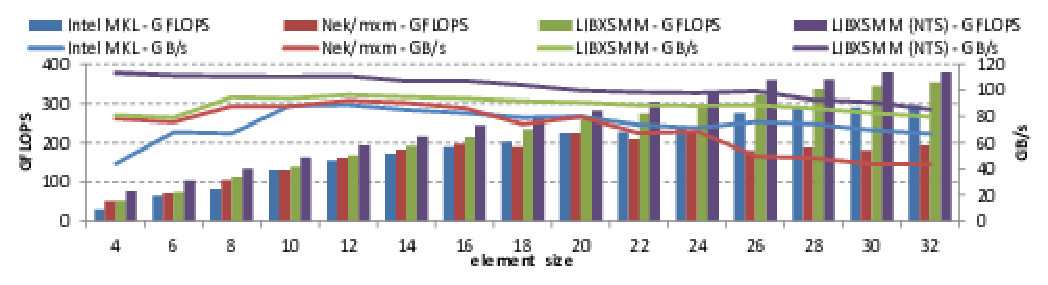
\includegraphics[width=1.0\textwidth]{gfx/axhm}
\caption{
Performance of the Helmholtz reproducer running on a single node of Shaheen for different implementation of small matrix multiplications. 
NTS denotes the usage of the non-temporal store optimized module.}
\label{fig:axhm}
\end{figure}

The performance numbers for the basis transformation on Shaheen are comparable to the Helmholtz operator and 
therefore not plotted. 
To summarize them, LIBXSMM-based GEMMs are the fastest and, due to higher computational demand, NTS are only important of for very small 1d sizes.
LIBXSMM is able to achieve 50\% of maximum floating-point performance for moderate orders.
LIBXSMM ranges from 4$\times$ faster than \texttt{mxm\_std} and Intel MKL at the smallest order to 40\% faster at the largest.


The performance of the Helmholtz kernel is representative of the basis transformations kernel on Mira as well.
To compare with Shaheen, \fref{axhm_mira} repeats the Helmholtz operator reproducer experiment
on a single node of Mira. 
IBM ESSL version 5.1.1 is used as the vendor library in place of Intel MKL.
In place of LIBXSMM, \texttt{mxm\_bgq}, which features QPX SIMD instructions, is used for the sizes that it supports.
When no QPX implementation is available, \texttt{mxm\_bgq} falls back to \texttt{mxm\_std}. 
Up to element size 16, Nek's \texttt{mxm\_std} and \texttt{mxm\_bgq} libraries are a better choice compared to IBM ESSL.
For larger element sizes (except 22 and 24) the performance is comparable.
However, the fraction of available bandwidth used is significantly worse than on Shaheen. 
Even at high element sizes, Shaheen is at 80\% bandwidth utilization with LIBXSMM and 50\% without, whereas Mira runs at 17\%.
The relative efficacy of \texttt{mxm\_bgq} on Mira, where available, highlights the strength of LIBXSMM: the ability to automatically issue the best available vector instructions at any size.


\begin{figure}[!t]
\centering
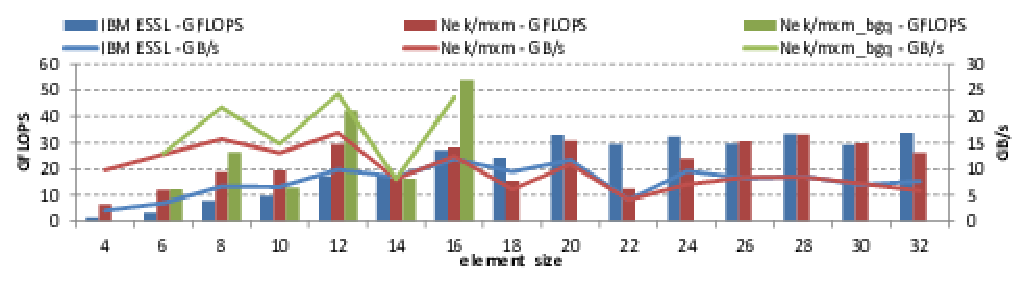
\includegraphics[width=1.0\textwidth]{gfx/axhm_mira}
\caption{
Performance of the Helmholtz operator reproducer running on a single node of Mira for different implementation of small matrix multiplications.}
\label{fig:axhm_mira}
\end{figure}

\fref{rstr} depicts corresponding performance numbers for the basis transformation reproducer in three use cases: a) unitary transformation from element size to element size, b) prolongation/dealiasing from 1d size to $(3/2)$ the element size, and c) restriction/aliasing from 1d size to (2/3) the element size.
Note that the $(3/2)$ factor implies some dimensions are significantly larger then the element size shown on the x-axis.

As with the Helmholtz reproducer, the LIBXSMM-based executions are the fastest and due to higher
computational demand; 
NTS are only important of for very small 1d sizes. 
LIBXSMM is able to achieve 50\% of maximum floating-point performance for medium sized orders
In direct comparison to \texttt{mxm\_std} and Intel MKL, the speed-up of LIBXSMM varies between close to 4$\times$ at very small order to roughly 40\% at very large order.

\begin{figure}[!t]
\centering
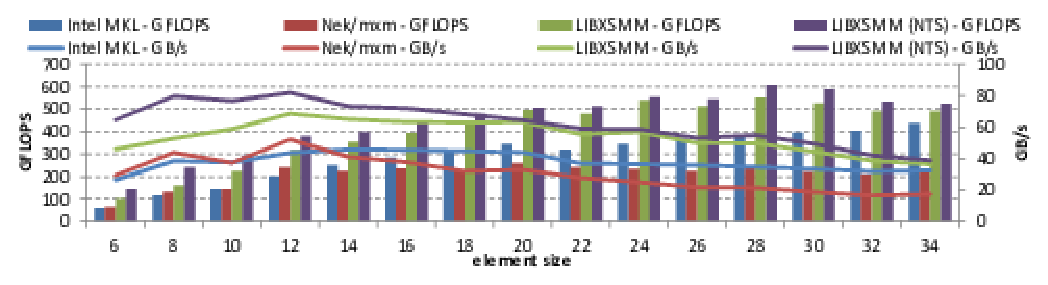
\includegraphics[width=1.0\textwidth]{gfx/rstr}   
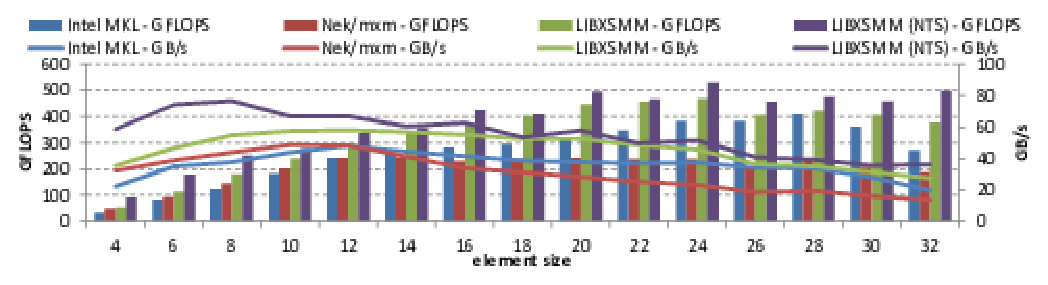
\includegraphics[width=1.0\textwidth]{gfx/rstr_fwd}
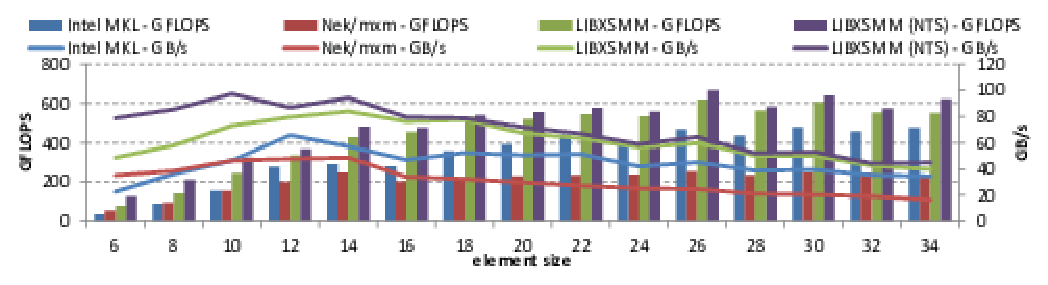
\includegraphics[width=1.0\textwidth]{gfx/rstr_rev}
\caption{Performance of the basis transformation reproducers using different implementation for the 
small matrix multiplications. NTS denotes the usage of the aforementioned non-temporal store optimized module. The top plot
shows the diagonalization in the local Poisson operator, the middle one the prolongation and the bottom one the restriction case.}
\label{fig:rstr}
\end{figure}

%Finally, the gradient reproducer's performance is plotted in \fref{grad}.
%The floating point load is very similar to Helmholtz, but only one element is read, instead of five, and three elements are written, %instead of one.
%While both are bandwidth bound, the higher write load makes gradient more sensitive to RFO.
%NTS doubles the performance in case of small and medium sized orders. 
%Therefore, without NTS, the high bandwidth cost masks the floating point cost and it does not matter which matrix-matrix routines are %used.
%Even so, LIBXSMM results in the fastest execution.
%
%\begin{figure}[!t]
%\centering
%\includegraphics[width=1.0\textwidth]{gfx/grad}
%\caption{Performance of the gradient operator reproducer using different implementation for the small matrix 
%multiplications. NTS denotes the usage of the aforementioned non-temporal store optimized module.}
%\label{fig:grad}
%\end{figure}


\section{Scenarios and Performance}
\label{sec:benchmarks}
\subsection{Architectures} \slabel{arch}

We run on two supercomputers: Mira at the ALCF and Shaheen XC40 at the KSL.
Mira is a IBM BlueGene/Q with 49,152 nodes.
Each node has 16 cores with 4 hardware threads per core and can support 204.8
GFLOPS and 30 GiB/s main memory bandwidth, measured by~\cite{McCalpin2007}.
Shaheen is a Cray XC40 with 6144 nodes.
Each node has two Intel\textsuperscript{\textregistered}
Xeon\textsuperscript{\textregistered} E5-2698v3 (code-named Haswell) processors
with 16 cores each and can support around 1177.6 GFLOPS and 101.6 GiB/s main memory bandwidth, measured by~\cite{McCalpin2007}.
Shaheen's cores therefore have 2.9$\times$ the floating point and 1.7$\times$ the memory bandwidth of Mira's BlueGene/Q cores.

\subsection{Single mode Rayleigh-Taylor instability}

The Rayleigh-Taylor instability (RTI) occurs when the pressure and density gradients point in opposite directions, as in the canonical case of a heavy fluid supported on top of a lighter fluid in a gravitational field.
The Rayleigh-Taylor growth rate is an increasing function of the wave-number, up to a viscous cutoff, making the smallest scales grow fastest.
Because energy is pumped into the system at small scales, the RTI is notoriously difficult to model numerically~\cite{Dimonte2004}.

The RTI describes how the dense fluid is pushed through and mixes with lighter fluid.
This dynamic mixing process is essential to the behavior of flows found in exploding stars~\cite{Bell2004}, the oceans and atmosphere~\cite{Linden1973}, and inertial confinement fusion.
In the latter case, dense plastic ablator is pushed into and mixed with the lighter hydrogen fuel.
The carbon-laden ablator radiates energy much more quickly than the fuel, reducing hot-spot temperature and preventing ignition.
The study of the RTI and related mixing is a priority research direction for inertial confinement fusion performance~\cite{Gocharov2012}.

Nek5000 and NekBox~\cite{NekBox} are used to model the incompressible Boussinesq equations, which approximate the RTI at low density contrasts:
\begin{align}
\frac{\partial u}{\partial t} + u \cdot \nabla u &= - \nabla p + \nu \nabla^2 u + \tilde{g} T \\
\frac{\partial T}{\partial t} + u \cdot \nabla T &= \alpha \nabla^2 T \\
\nabla \cdot u &= 0,
\end{align}
where $T$ is a scalar that can be interpreted as a temperature, 
in which case $\alpha$ is the thermal diffusivity 
and $\tilde{g}$ is the product of the gravitational acceleration and the thermal expansion coefficient.

The single-mode Rayleigh-Taylor instability (smRTI) restricts the initial perturbation of the interface to be sinusoidal, and is generally considered in periodic span-wise boundary conditions:
\begin{equation} \elabel{IC}
T(x,y,z,0) = A\cdot \text{erf}\left[\frac{z + a_0 \cos(2 \pi x/\lambda) \cos(2 \pi y/\lambda)}{\delta}\right],
\end{equation}
where $A \in (0,1]$ is the Atwood number,
$\lambda$ is the wavelength, 
$a_0$ is the initial interface amplitude, and
$\delta$ is the initial interface width.
This simplification allows the problem to be defined by only two dimensionless numbers in the limit of $a_0, \delta \rightarrow 0$, the Grashof number (Gr) and the Prandtl number (Pr):
\begin{equation}
\text{Gr} = \frac{A \tilde{g} \lambda^3}{\nu^2},  \qquad \text{Pr} = \frac{\nu}{\alpha}.
\end{equation}

Even under these simplifications, the late-time behavior is not well understood.
Experiments are prone to spurious low-wavelength modes that dominate the dynamics at late times, while the cost of direct numerical simulations is quadratic with the domain's aspect ratio.

It would be valuable to systematically sample the Grashof-Prandtl space with high fidelity simulations at late-time/high-aspect-ratio to better inform experimental design and model development.
Such a study would be very expensive, so it is important to select a cost-minimizing strategy.

We take this problem, the selection of a cost-minimizing strategy for the late-time smRTI, as our motivation.
In addition to the isolated reproducers discussed in \sref{implementation}, we present NekBox application benchmarks based on smRTI with typical Nek settings.
The aim of these benchmarks is to identify minimum cost discretizations that attain a given accuracy.

The benchmarks are conducted for combinations of the element size taken from $\{4, 6, 8, 10, 12, 14, 16, 32\}$ and span-wise mesh size taken from $\{2, 4, 8, 12, 16, 24, 32, 48, 64, 96, 128\}$.
The total number of points ranges from around 1 million to 4 billion.
The problem is weak-scaled: the number of elements per rank is chosen as to consume approximately half of the available main memory, or around 16k and 262k points per rank on Mira and Shaheen, respectively.
The problems are constrained to fill an integer number of nodes, which puts a lower bound on the mesh size and excludes some cases that would partially fill nodes.
The domain is a box with dimension $[0,.5]^2 \times [-1,1]$, and the elements are cubic.
The span-wise boundary conditions are symmetric and the vertical boundary conditions are no-slip in velocity and no-flux (insulating) in the scalar.
The initial condition is stationary in velocity with a scalar given by \eref{IC}, the Grashof number is 17,324, and the Prandtl number is 1.
The timestep is calculated based on a Courant number of $0.4$, which scales linearly with the number of elements and quadratically with the size of the element due to the spacing of the GLL nodes.
The Courant condition is defined only in a linear limit, so during the initial exponential growth regime the Courant number is computed using the stagnation velocity, $\sqrt{A \tilde{g}/(\pi \lambda)}$.


Outputs are written at regular intervals in simulated time, constant across problem sizes.
Therefore, smaller problems perform a greater share of I/O, as is the common case in CFD.
Nek5000 and NekBox write separate files for separate ranks.
The number of ranks that participate in I/O is a fixed proportion of the total number of ranks.

\begin{figure}
\begin{subfigure}[b]{0.25\textwidth}
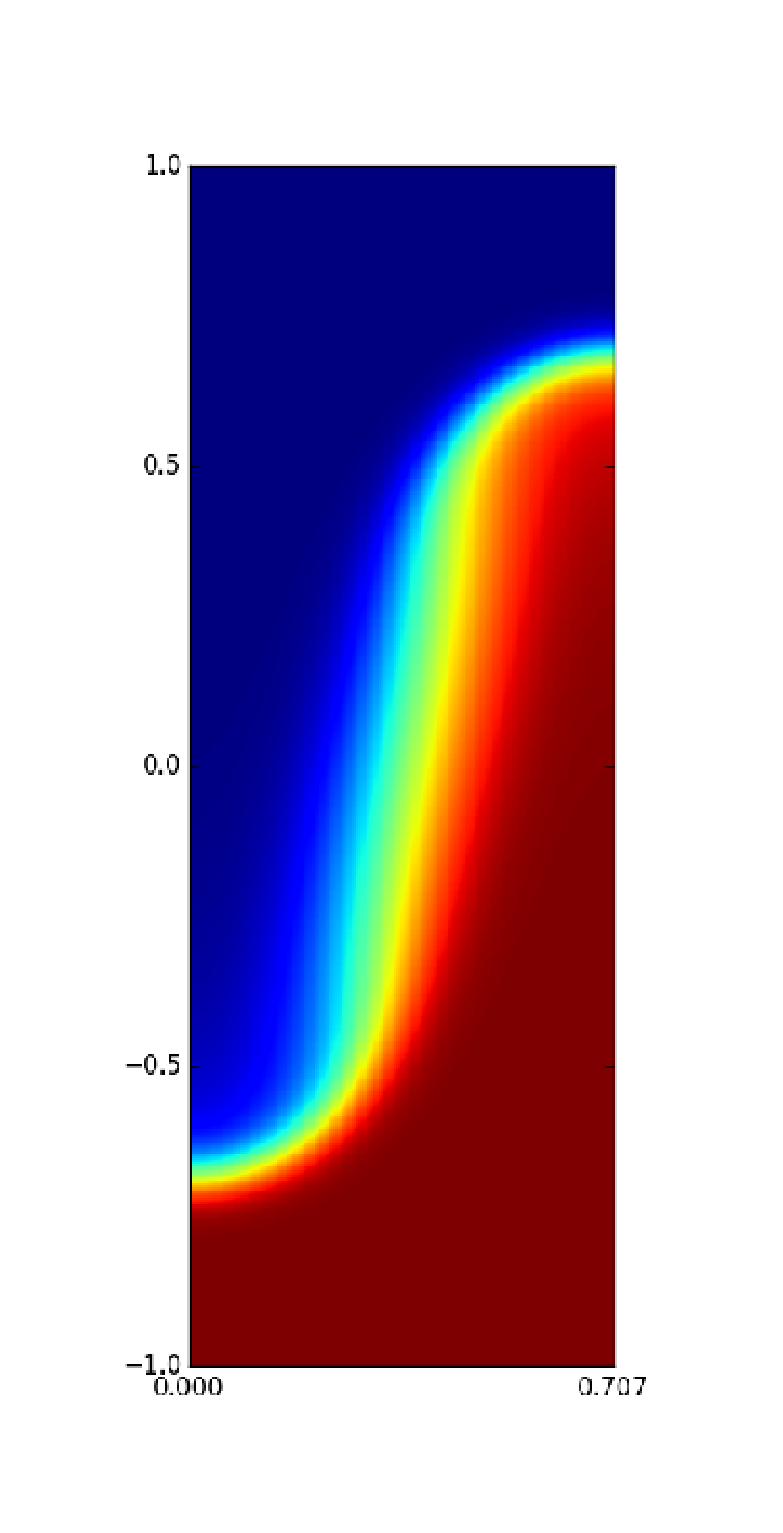
\includegraphics[width=0.25\textwidth]{gfx/cnv_o16_e32-t_yz-0033}
\end{subfigure}
\begin{subfigure}[b]{0.25\textwidth}
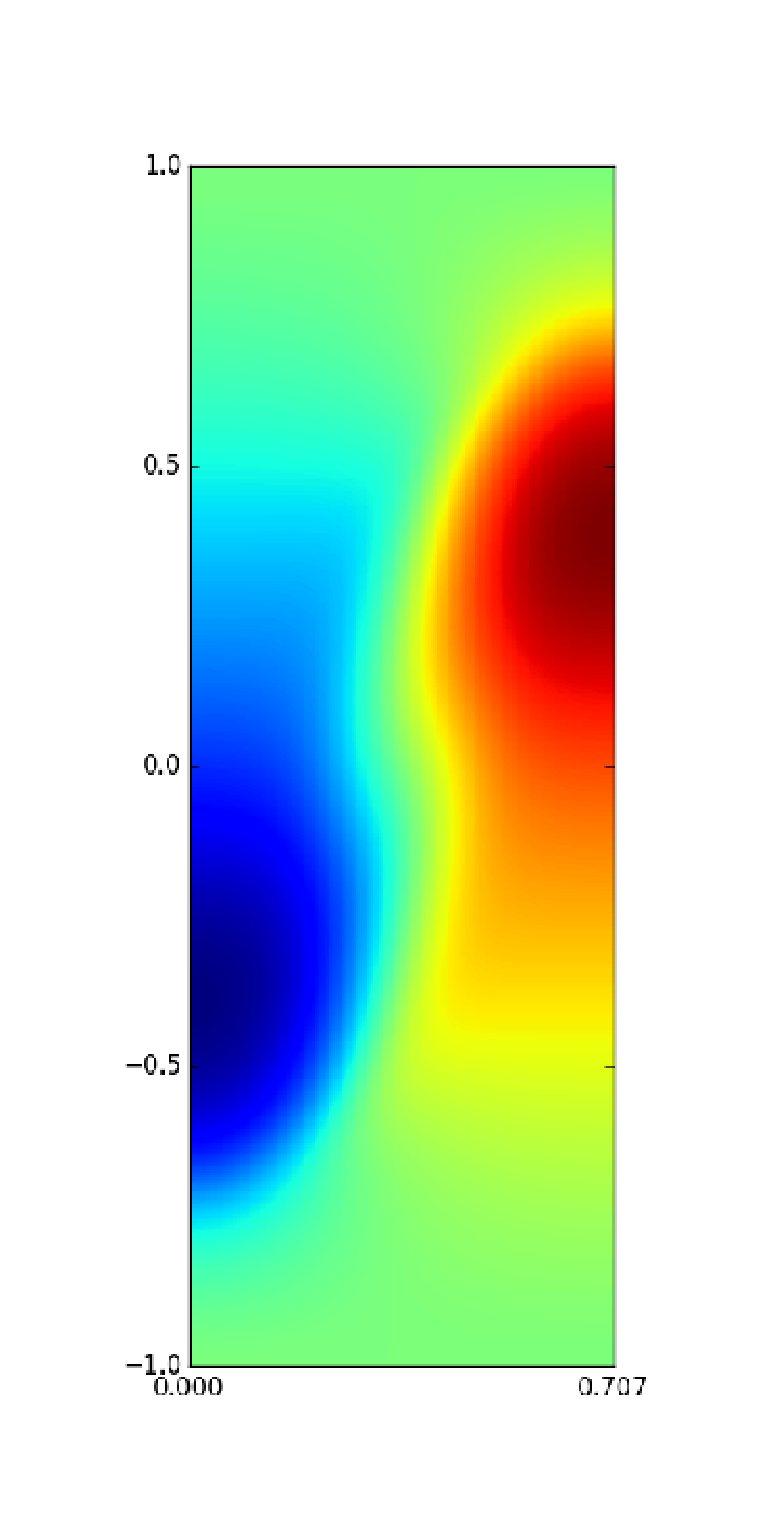
\includegraphics[width=0.25\textwidth]{gfx/cnv_o16_e32-w_yz-0033}
\end{subfigure}
\begin{subfigure}[b]{0.25\textwidth}
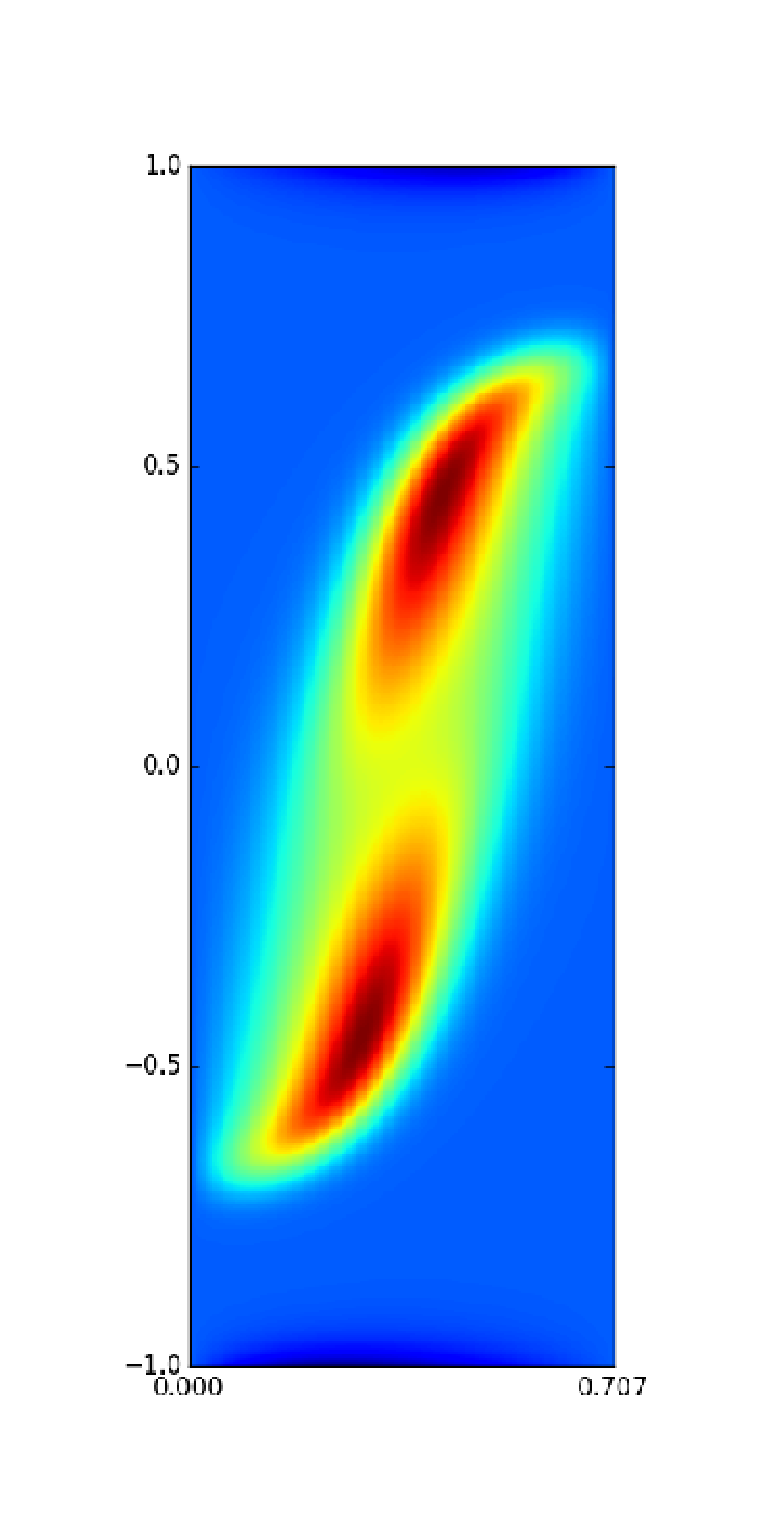
\includegraphics[width=0.25\textwidth]{gfx/cnv_o16_e32-vorticity_yz-0033}
\end{subfigure}
\begin{subfigure}[b]{0.25\textwidth}
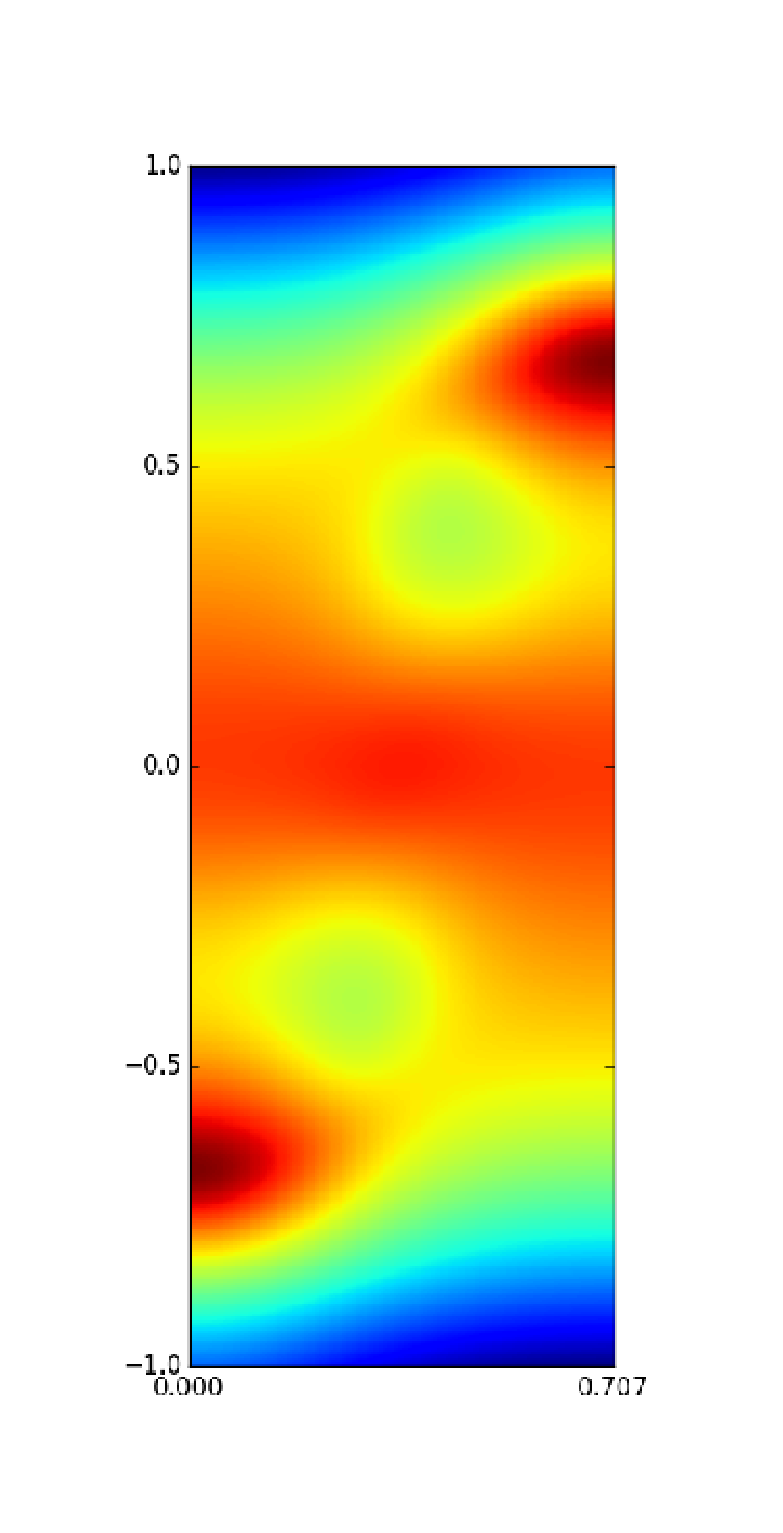
\includegraphics[width=0.25\textwidth]{gfx/cnv_o16_e32-p_yz-0033}
\end{subfigure}
\caption{ \flabel{slices}
Scalar, velocity, vorticity, and pressure fields at end of simulation.
}
\end{figure}

Slices of the end of the simulation are shown in \fref{slices}.
Two observables are calculated in post-processing: the \textit{bubble height} and the \textit{mix volume}:
\begin{equation} \elabel{observe}
H = \sup \left\{ z : \min_{x,y} ~ T(x,y,z) < T_0\right\}, \qquad
\Theta = \int \left|T - T_0\right| dV, 
\end{equation}
where $T_0$ is the volumetric average temperature.
These two observables are common to smRTI models and lie at opposite ends of the locality spectrum: 
the bubble height is defined by the neighborhood of the bubble tip while the mix volume is an integral over the entire domain.
The root mean square error in each observable is computed over all the outputs.


\subsection{Time to accuracy}

\begin{figure}
\begin{subfigure}[t]{0.49\textwidth}
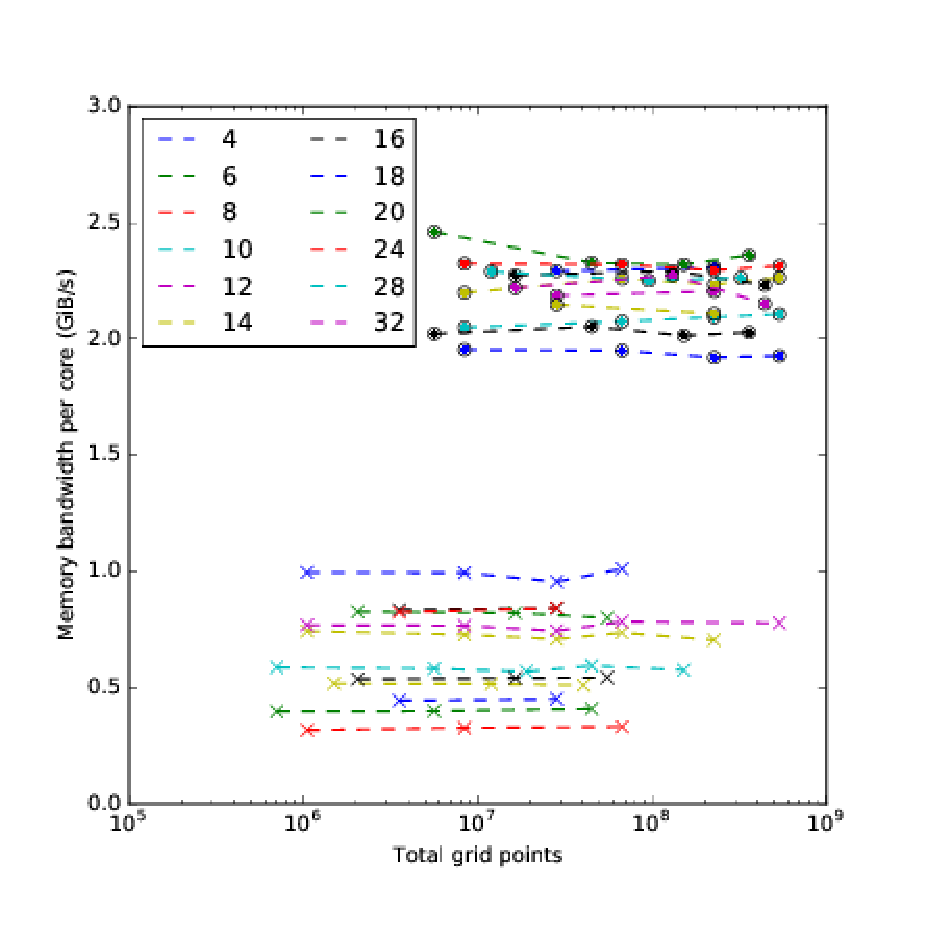
\includegraphics[width=0.49\textwidth]{gfx/combined-bw}
\caption{Bandwidth}
\end{subfigure}
\begin{subfigure}[t]{0.49\textwidth}
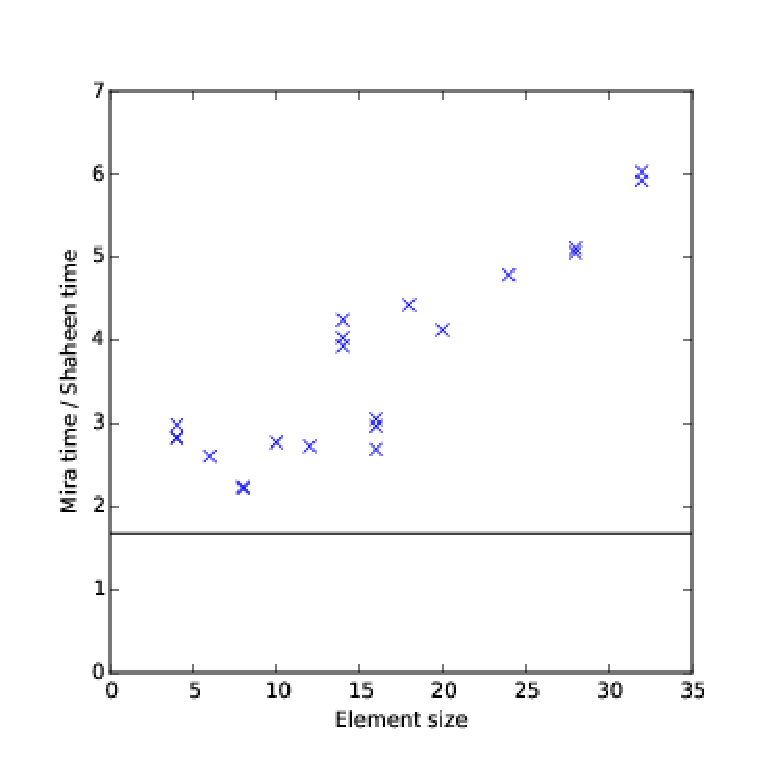
\includegraphics[width=0.49\textwidth]{gfx/mira_vs_haswell}
\caption{Ratio}
\end{subfigure}
\caption{ \flabel{bwcomp}
Weak scaling of bandwidth on Shaheen and Mira.
In (a), Circles and crosses indicate memory bandwidth per core on Shaheen and Mira, respectively, vs the problem size labeled by element size.
In (b), the ratio of the bandwidths are shown vs element size for common discretizations.
The solid line indicates ratio of STREAM memory bandwidth.
}

\end{figure}

For each simulation, we compute the FLOP rate and aggregate memory bandwidth.
NekBox includes explicit FLOP and memory operation counters and timers in the most performance critical regions of the code.
Memory operations are counted assuming single-element intermediate data stays in cache, and therefore does not contribute to main memory bandwidth.
These counters are consistent with those used in the reproducers.
The whole application is not covered, so the counters can be considered lower bounds on the whole-application performance.

The attained memory bandwidth per core on Shaheen and Mira are plotted in \fref{bwcomp}.
On Shaheen, bandwidth is constant with respect to the number of elements and a weak function of the order, ranging from around 65 to 75\% of peak.
On Mira, bandwidth is still constant with respect to the scale, but varies more strongly with polynomial order, especially at orders greater than 16 and those not divisible by 4.
It ranges from around 15 to 50\% of peak.
The \texttt{mxm\_bgq} library, discussed in \sref{implementation}, is used, resulting in performance spikes at QPX-supported orders, e.g. 8.

\begin{figure}
\begin{subfigure}[t]{0.49\textwidth}
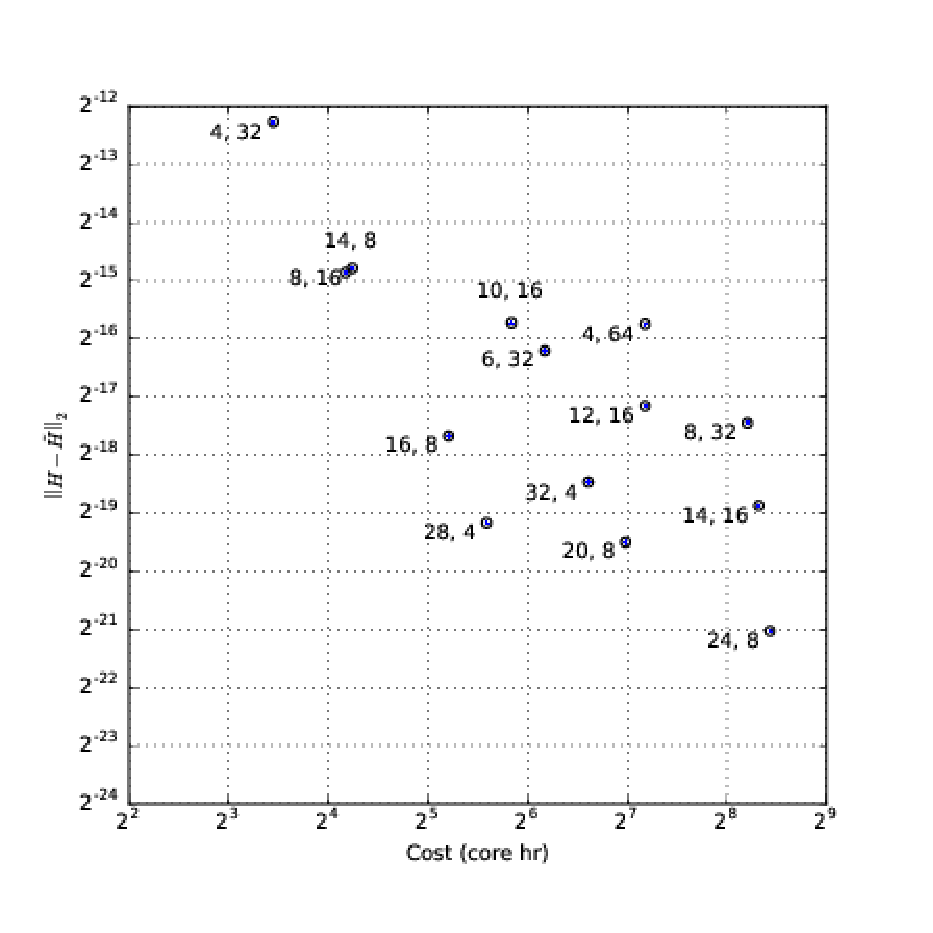
\includegraphics[width=0.49\textwidth]{gfx/shaheen_H}
\caption{Shaheen}
\end{subfigure}
\begin{subfigure}[t]{0.49\textwidth}
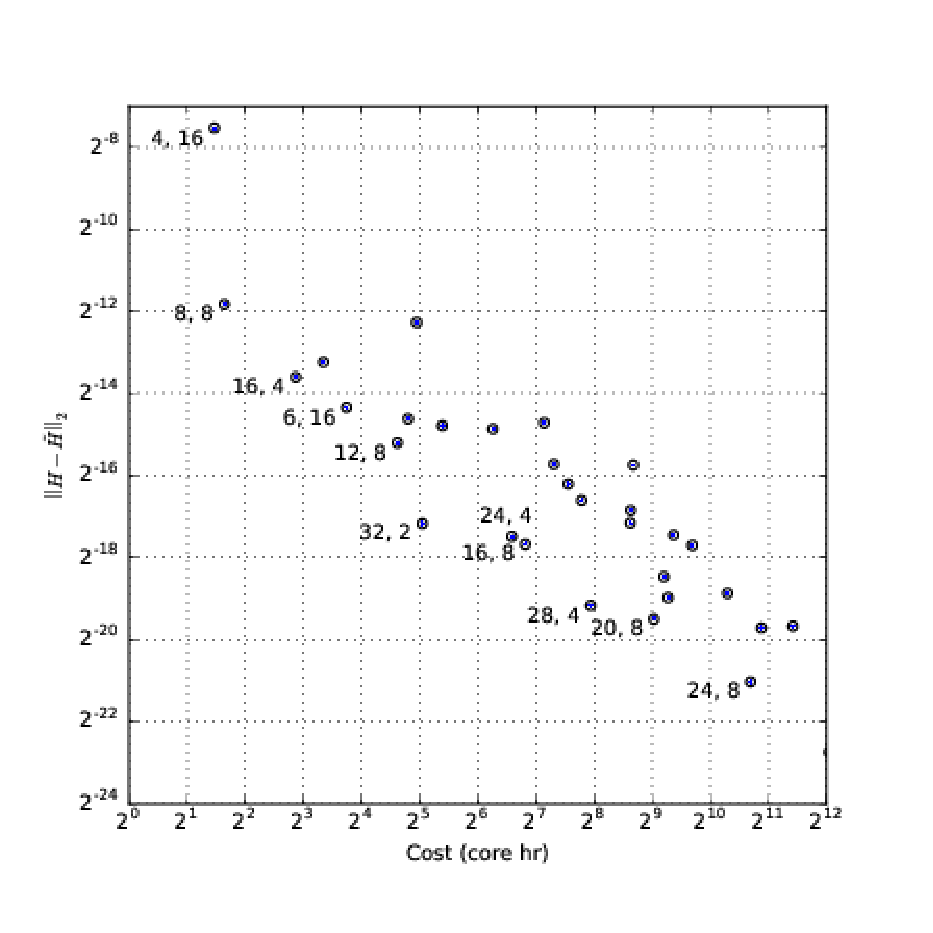
\includegraphics[width=0.49\textwidth]{gfx/mira_H}
\caption{Mira}
\end{subfigure}

%\subfloat[][Error wrt $dt$]{\includegraphics[width=0.33\textwidth]{gfx/cnv_wrt_t}}
%\subfloat[][Shaheen ($\Theta$)]{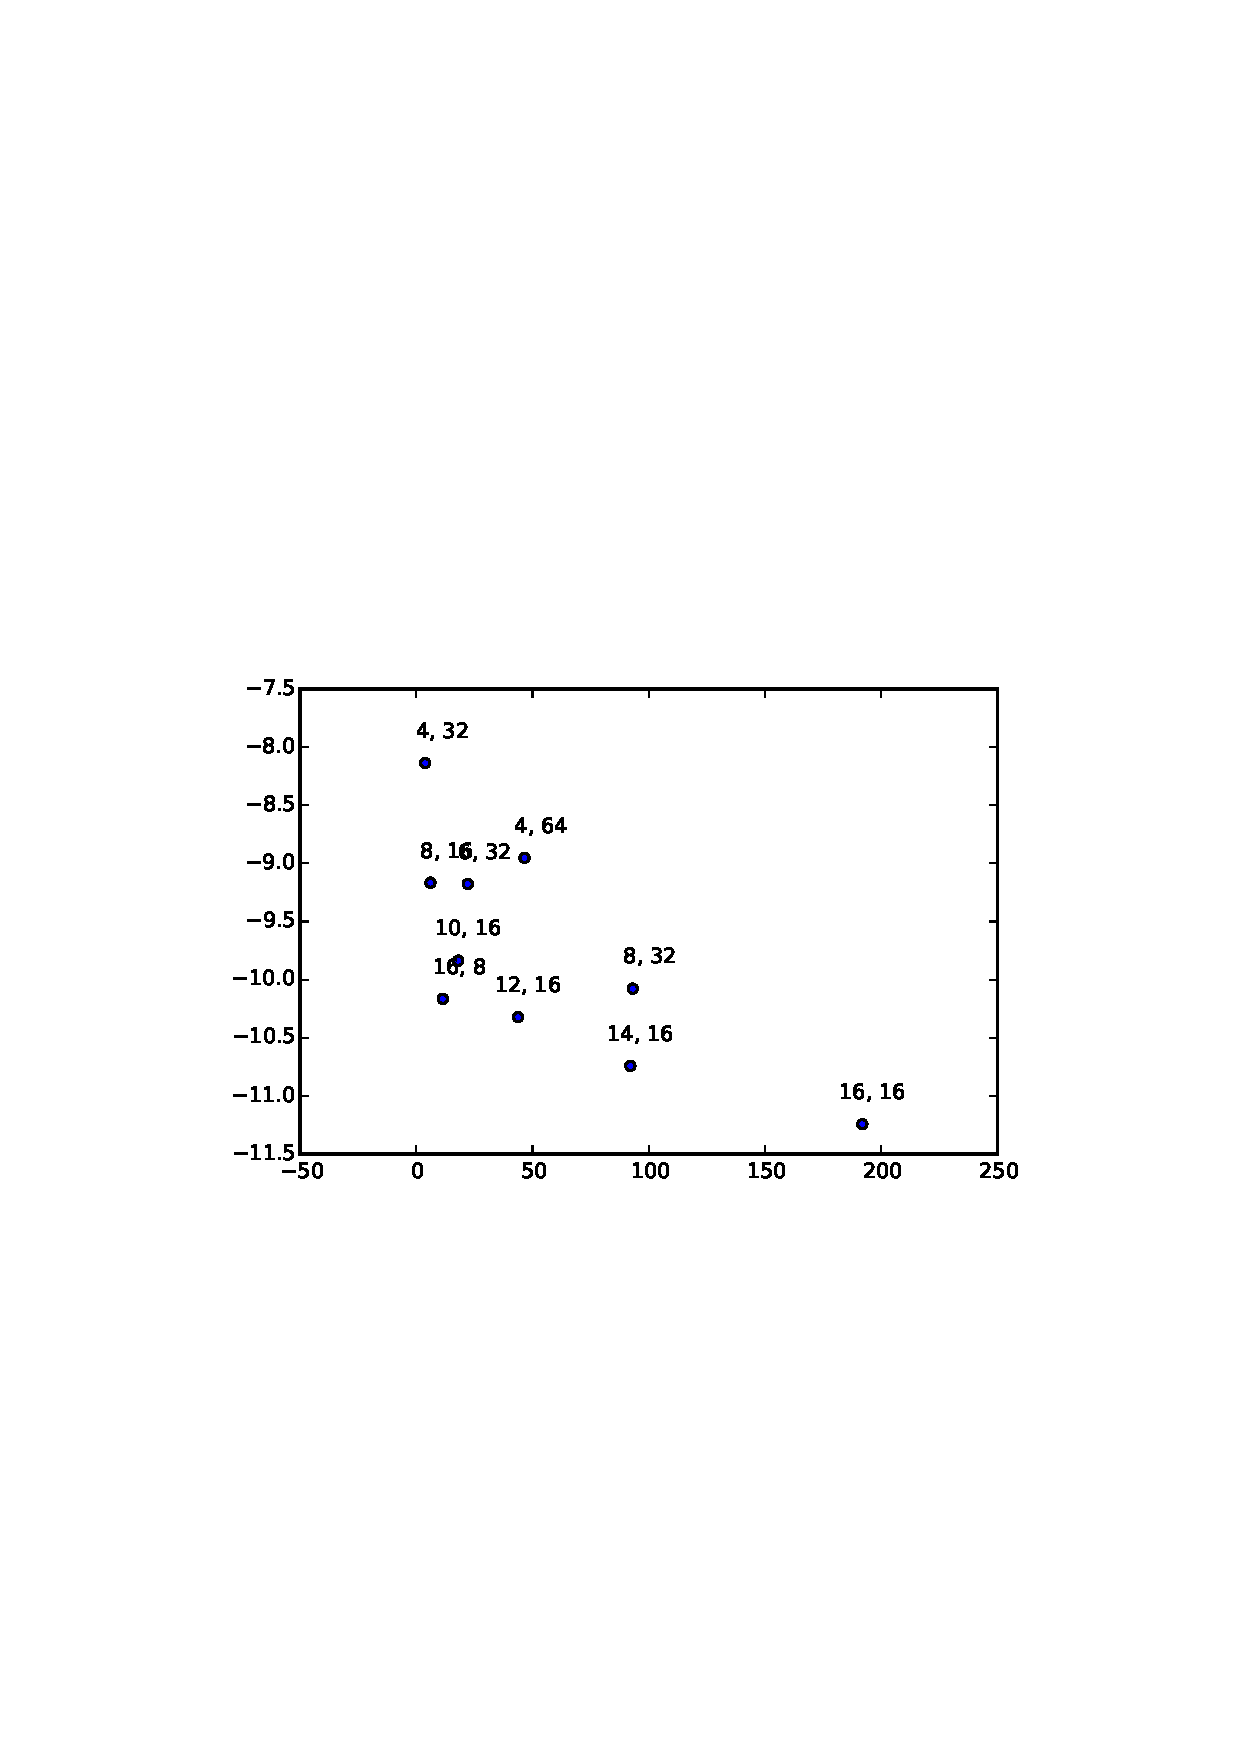
\includegraphics[width=0.5\textwidth]{gfx/shaheen_A}}

%\subfloat[][Mira ($\Theta$)]{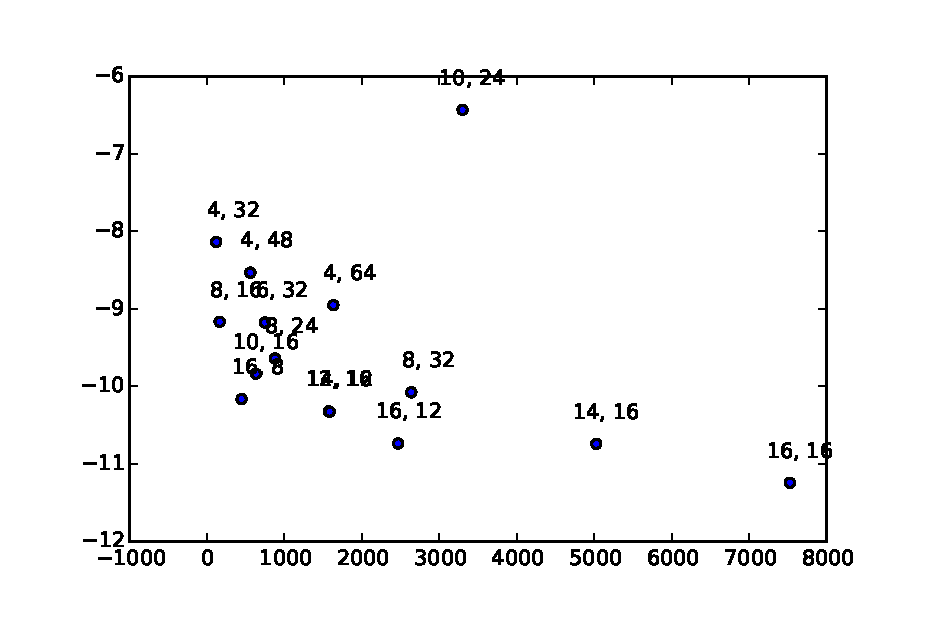
\includegraphics[width=0.5\textwidth]{gfx/mira_A}}

\caption{ \flabel{frontier}
Error with respect to bubble height, \eref{observe}, vs. the computational cost, in processor hours, on Shaheen (a) and Mira (b).
Points are labeled as $(p+1, e)$ pairs, where $p$ is the order, $p+1$ is the element size, and $e$ is the number of elements in one dimension.
More runs are present on Mira due to the smaller BGQ nodes evenly dividing more problem sizes.
}
\end{figure}

The accuracy is plotted versus the computational cost for a variety of discretizations in \fref{frontier}.
The error in bubble height and mix volume are strongly correlated, so only the error in the height is plotted.
As expected, doubling the the spectral order while keeping the number of elements fixed, e.g. $(4,32) \rightarrow (8,32)$ and $(8,8) \rightarrow (16,8)$, significantly improves the accuracy, but also increases the cost by 16-32$\times$.
The first 8$\times$ is due to an increase in the number of degrees of freedom, the next 2$\times$ is due to the shorter timestep, and, when compute-bound, the final 2$\times$ is due to an increase in the floating point load.
Doubling the spectral order while keeping the number of points fixed, e.g. $(16, 8) \rightarrow (32,4)$  and $(8,8) \rightarrow (16,4)$, increases the cost by 2-4x, as expected, but also improves the accuracy.
Doubling the spectral order while halving the number of points in each direction, e.g. $(8,32) \rightarrow (16,8)$ and $(14, 16) \rightarrow (28, 4)$, reduces the cost by 4-8$\times$ while maintaining or slightly improving the accuracy.

We define the \emph{efficiency frontier} as the set of discretizations that minimize computational cost for fixed accuracy or, equivalently, minimize error given fixed computational cost.
The efficiency frontiers on Mira and Shaheen are comprised of discretizations with very high orders, given our constraints.
The most efficient schemes are those with element size greater than 16, except for very low accuracy simulations.

\begin{comment}

\subsection{Order-independent timestepping}
\begin{figure}
\begin{subfigure}[t]{0.33\textwidth}
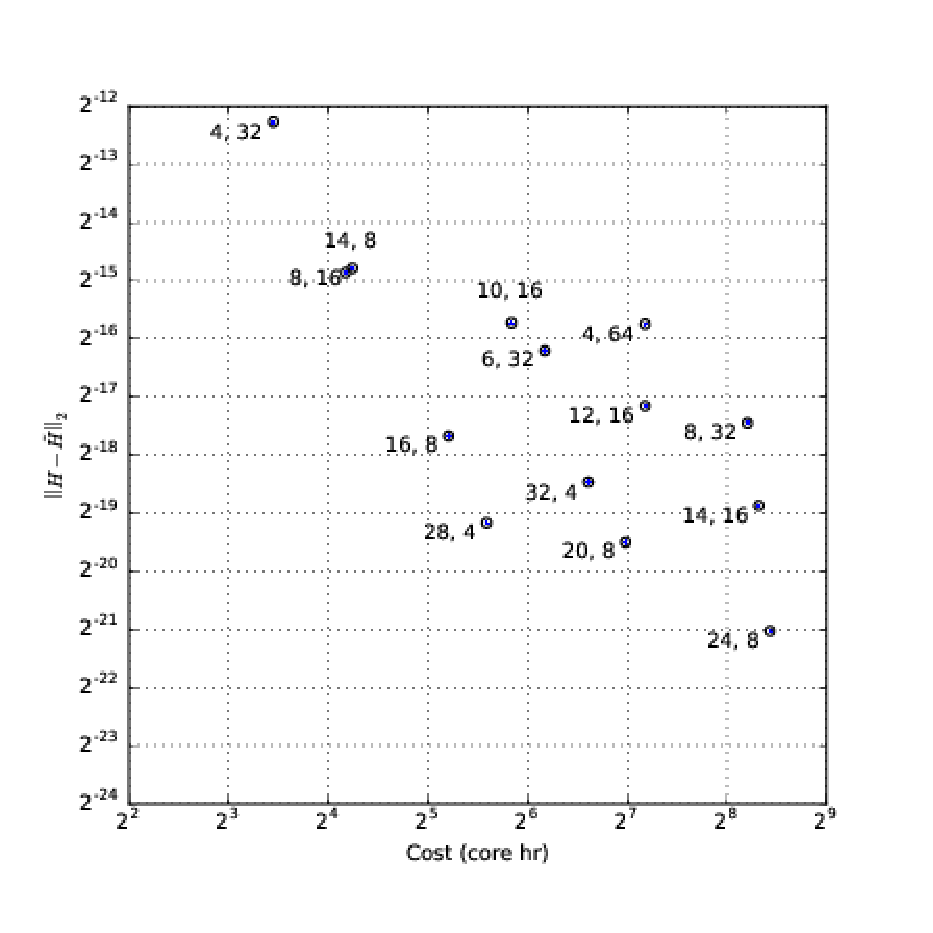
\includegraphics[width=0.49\textwidth]{gfx/shaheen_H}
\caption{Shaheen}
\end{subfigure}
\begin{figure}
\begin{subfigure}[t]{0.33\textwidth}
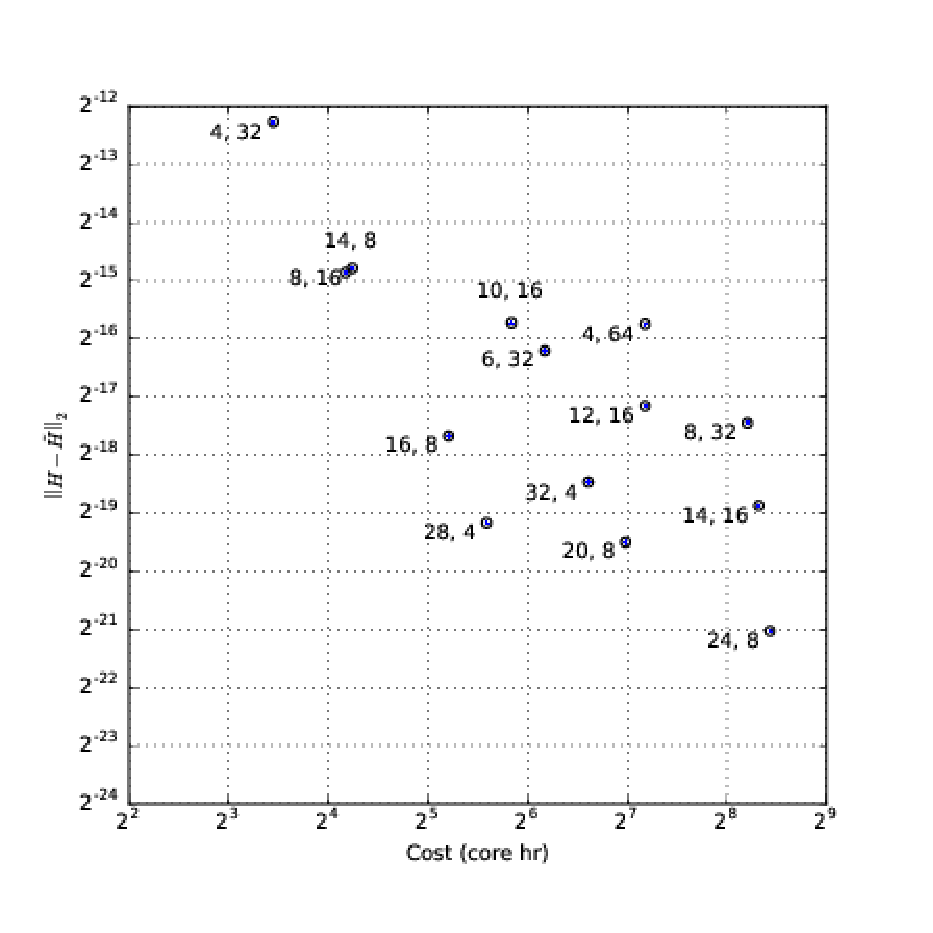
\includegraphics[width=0.49\textwidth]{gfx/shaheen_H}
\caption{Mira}
\end{subfigure}
\begin{figure}
\begin{subfigure}[t]{0.33\textwidth}
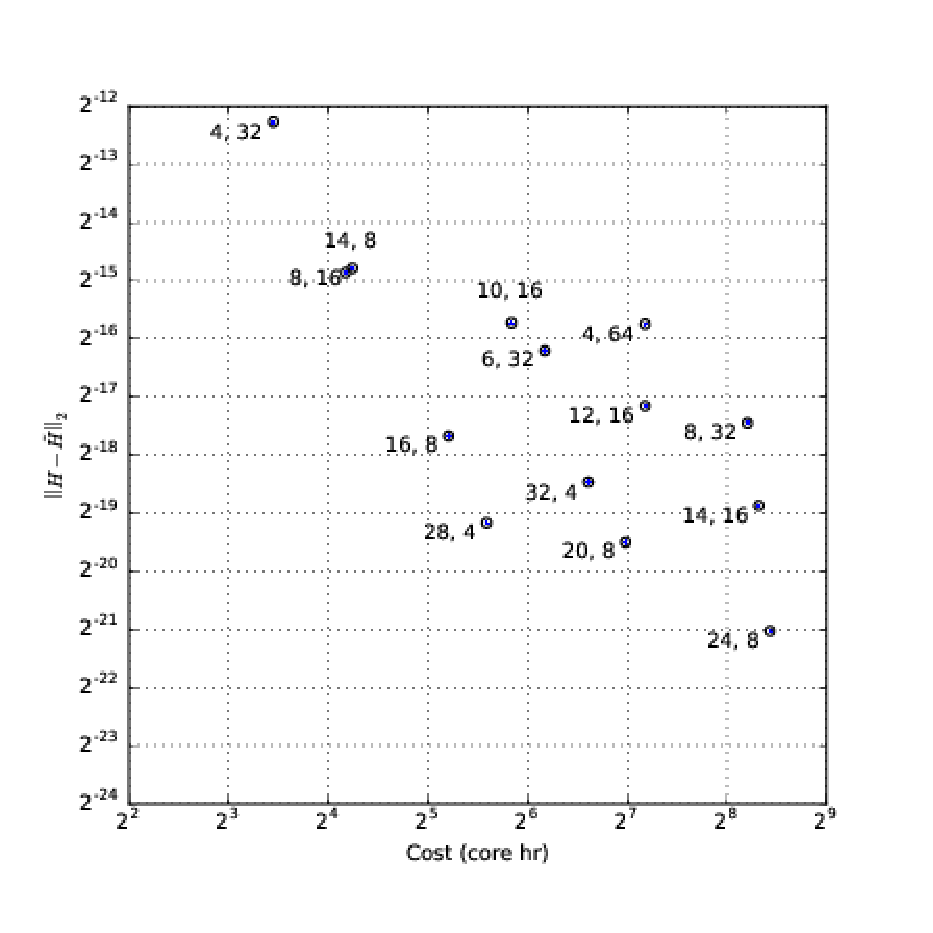
\includegraphics[width=0.49\textwidth]{gfx/shaheen_H}
\caption{Cost vs DOF}
\end{subfigure}



	\subfloat[][Shaheen]{\includegraphics[width=0.33\textwidth]{gfx/shaheen_cfl_H}}
\subfloat[][Mira]{\includegraphics[width=0.33\textwidth]{gfx/mira_cfl_H}}
\subfloat[][Cost vs DOF]{\includegraphics[width=0.33\textwidth]{gfx/perf_vs_dof}}
%\subfloat[][Shaheen ($\Theta$)]{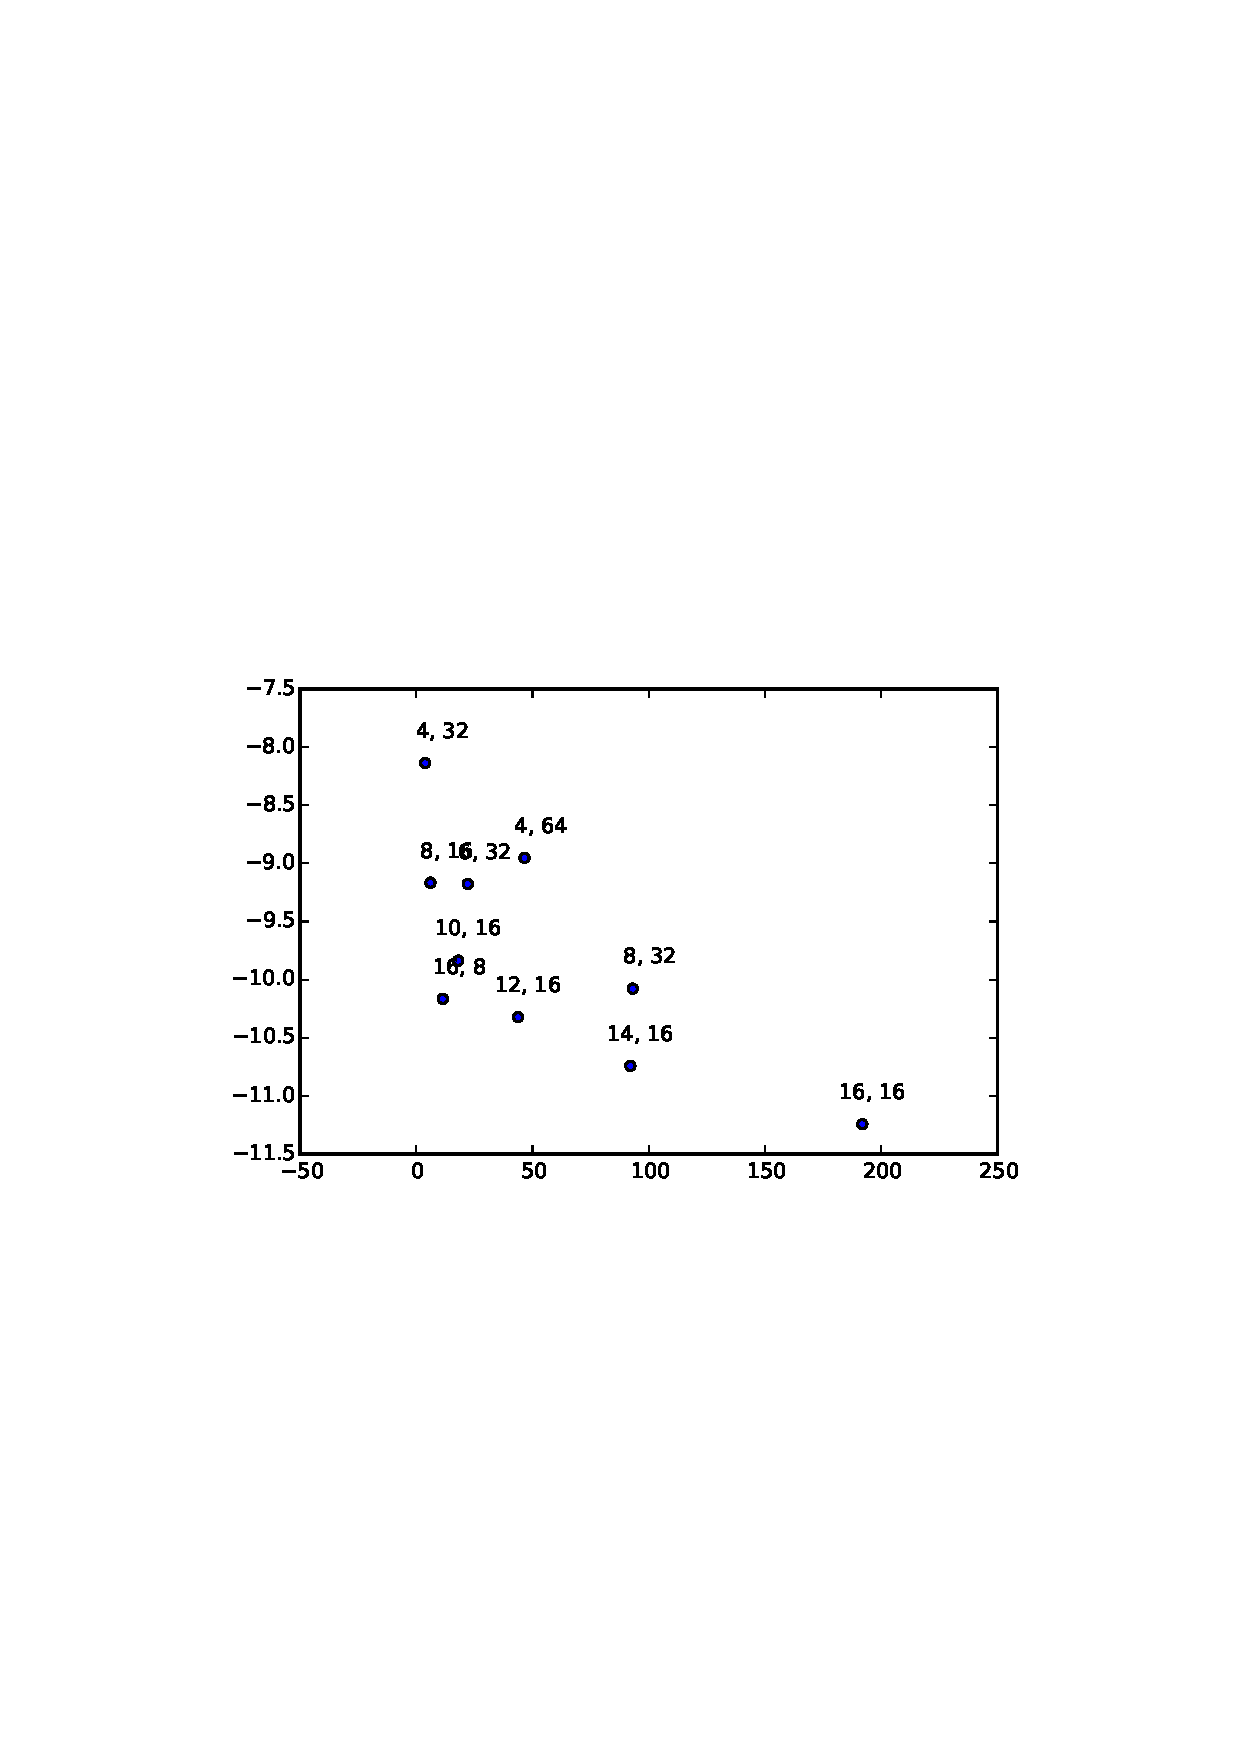
\includegraphics[width=0.5\textwidth]{gfx/shaheen_A}}

%\subfloat[][Mira ($\Theta$)]{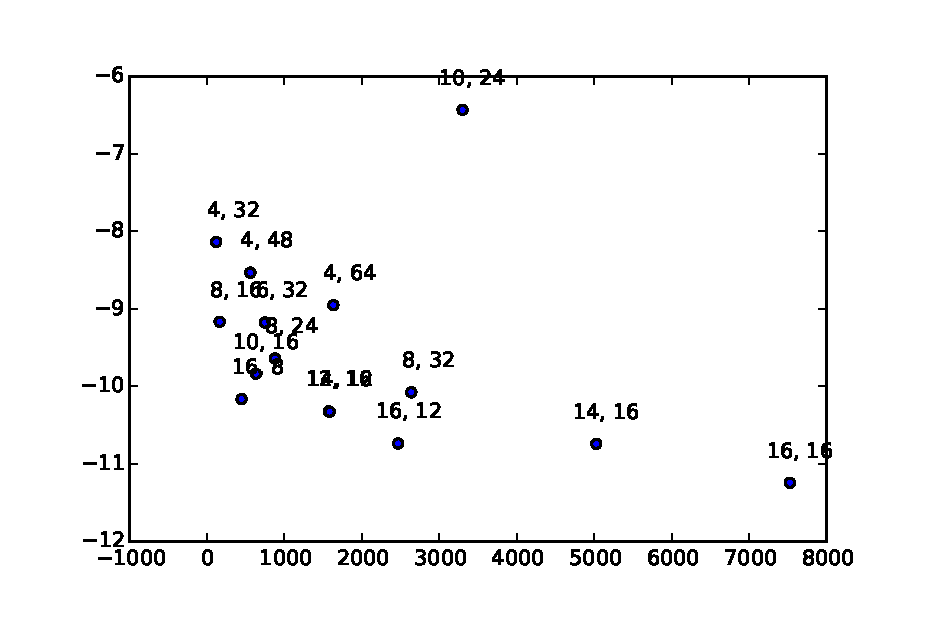
\includegraphics[width=0.5\textwidth]{gfx/mira_A}}

\caption{ \flabel{cfl3}
Error with respect to bubble height, \eref{observe}, vs. the computational cost, in processor hours, on Shaheen (a) and Mira (b).
Cost vs. total degrees of freedom (c), with circles from Mira and crosses from Shaheen.
In all cases, the ratio of timestep to maximal velocity is held fixed to match the CFL condition $C = 0.4$ in the (32,8) case, which sets the temporal error floor at the solid black line in (a) and (b).
}
\end{figure}

When using high order methods, there is often a gap between the convergence rate or the spatial and temporal discretizations.
To achieve high accuracy, it is necessary to reduce the timestep below the CFL stability condition.
Doing so decouples the number of timesteps from the element size.
Now, the computational cost depends on the order, for fixed total points, only through an increase in arithmetic intensity.
If the calculation is bandwidth-bound, then high order should come at no marginal cost.
If the calculation is compute-bound, then high order should come at linear cost, in return for exponential spatial convergence.

To demonstrate this, we reduce the time step to that of the $(32,8)$ discretization in the previous section by reducing the CFL number according to the spatial discretization.
This gives us a bound on the temporal error in $H$ of $2\times 10^{-6}$.
\fref{cfl3} plots the accuracy vs the computational cost, as in \fref{frontier} but with order-independent timestepping, along with the cost vs degrees of freedom.
We see that the most efficient calculations, those that minimize cost for a given error, are all very high order.
The cost is a strong function of the number of degrees of freedom and a weak function of the order.
On Shaheen in particular, the dependence of the cost on the order seems to be in the noise, all
runs took roughly the same computing time, independent from the chosen order.
\end{comment}

\begin{comment}
\subsection{Discussion}

\subsubsection{Time to solution}

Here, we have considered computational cost in the high-throughput context: the consumption of computational resources as measured in core hours.
Alternatively, one could consider the low-latency context: the minimum time to solution, i.e. the strong-scaling limit.
In this limit, we care about the number and computational duration of time iterations.

If we

This analysis can fail in at least three ways: a) we could saturate the network before we hit latency limits, which is unlikely given that Nek is predominantly nearest-neighbor; b) we could hit the coarse grain parallelism limit before we hit latency limits; or c) the number of iterations in the solvers could increase or decrease.

On low-latency networks, Nek5000's strong scaling limit is known to be of order 1000 grid points.
NekBox reduces the communication load, so its limit could be lower.
Therefore we expect to hit (b) at polynomial order between 10 and 16.
\end{comment}

\subsection{Whole application performance}

\begin{figure}[!t]
\centering
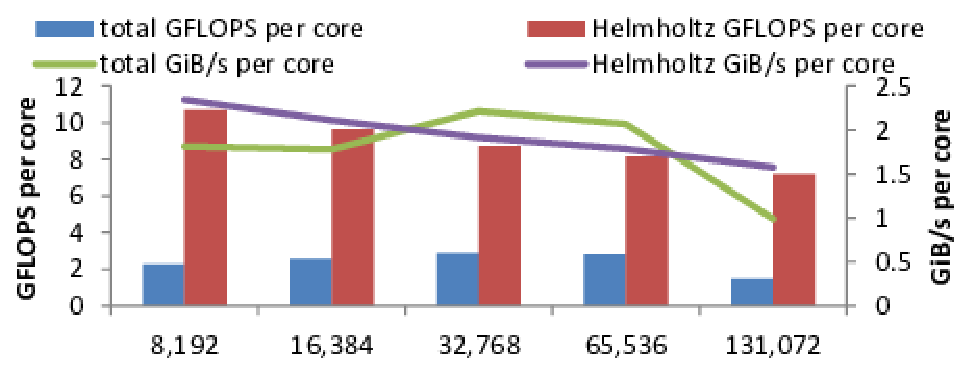
\includegraphics[width=0.55\textwidth]{gfx/shaheen_strong}
~
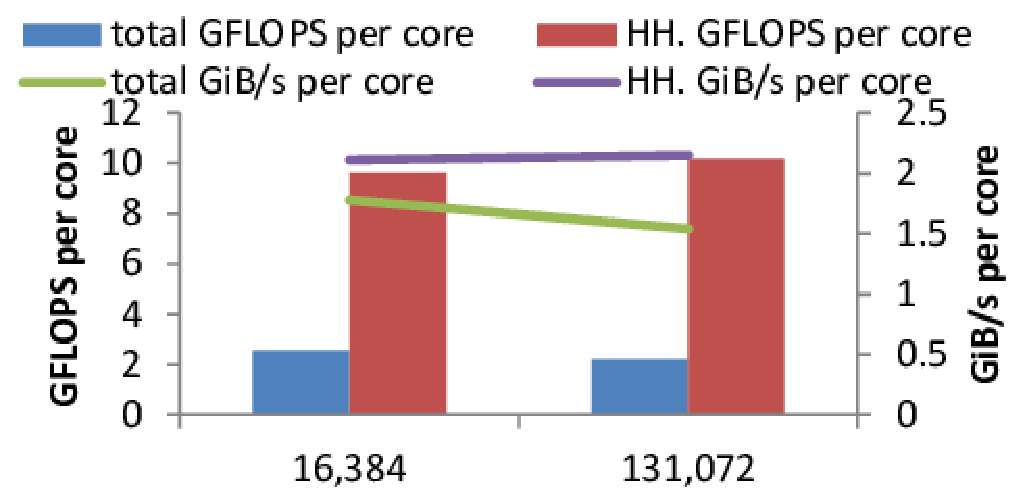
\includegraphics[width=0.42\textwidth]{gfx/shaheen_weak}
\caption{Strong scaling (left) and weak scaling (right) on Shaheen on up to 131,072  cores (2/3) of the full 7 PFLOPS machine using 
an element size of 32.
To avoid log plots we show per-core performance.}
\label{fig:shaheen_scaling}
\end{figure}

To date, our largest calculation on Shaheen occupied 131,072 cores as depicted in Fig.~\ref{fig:shaheen_scaling}
for element size 32.
NekBox achieved 197 TiB/s memory bandwidth and 290 TFLOPS in weak scaling.
This corresponds to 47.8\% of peak memory bandwidth sustained over the entire application at high order.
In case of strong scaling these numbers are slightly lower with 130 TiB/s and 195 TFLOPS. 
%This is true for both, weak and strong scaling, as Shaheen uses dynamic  node-level power capping, that kicks 
%in when more than about 1/3 of the machine is used~\cite{pedretti2015early}. This cap is most likely caused by
%the high demand of compute and bandwidth of the Helmholtz as this phase is still scaling and achieves 
However, the Helmholtz operator, as the most compute intense sub-routine, is able to achieve
up to 0.94\,PFLOPS in strong and 1.33\,PFLOPS
 in weak-scaling on 131,072 cores. %\footnote{We are currently working together with KSL to root-cause the
%power capping issues. Due to the holidays this was not possible at submission deadline.}
We also consider 65,536 cores runs, occupying 1/3 of Shaheen.
These runs achieved at least 135.6 TiB/s memory bandwidth and 184.9 TFLOPS.
This corresponds to 67.5\% of peak memory bandwidth sustained over the entire application at high order.
Finally, extrapolating to full machine, NekBox would reach at least 406.8 TiB/s and 554.6 TFLOPS. At the same scale,
a weak scaling of the Helmholtz operator would result into 1.9\,PFLOPS out of 7\,PFLOPS performance.





\section{Conclusion}
\label{sec:conclusion}
NekBox enhanced by LIBXSMM generated kernels on Shaheen XC40 executes the performance critical, order-dependent components of Nek above 80\% of peak memory bandwidth.
For comparison, compiled code on the BlueGene/Q architecture is only able to
reach 50\% of peak and for many polynomial orders operates around 30\%.
Therefore, despite only having 1.7$\times$ the memory bandwidth, Shaheen's cores
outperform Mira's cores by 3-6$\times$, with the greatest improvement at high
order and for sizes that are not divisible by the vector width, 4 in this case.
NekBox is able to scale 67.5\% utilization rates to 65,536 cores on Shaheen.

%, beyond which power throttling reduces efficiency by a factor of 2 overall. 
%However, the Helmholtz operator is relatively unaffected and able to achieve a PFLOPS of performance on 131,072 cores.

For the smRTI, the efficiency frontier, i.e., the discretizations that minimize
cost given accuracy or minimize error given cost, have polynomial orders between 15 and 31, higher than are typically used in spectral element schemes.
The presence of high order schemes on the efficiency frontier can be understood by the combination of two effects.
First, the increase in arithmetic intensity is hidden by the imbalance between floating point capabilities and memory bandwidth, providing high order at no marginal cost on a per time step basis.
Second, higher order schemes with fewer degrees are freedom are more accurate than lower order schemes with more degrees of freedom.
It is generally possible to maintain accuracy by increasing the order while decreasing the total degrees of freedom, and, consequently the total cost.

Generally the order should be chosen to be at least large enough to saturate the floating point capabilities of the architecture in the order-dependent kernels, because increasing the order to that point significantly improves accuracy at no marginal computational cost.
On BlueGene/Q, this mark is polynomial order 15, while on the Cray XC40 it is 31.

For many problems and observables, the calculation may additionally benefit from increasing the order until just before single-element operations spill out of cache.
The improvement in accuracy is exponential with the polynomial order, so the degrees of freedom needed to achieve a level of accuracy can decrease.
The increase in the cost with respect to order for compute-bound orders is linear, so if the decrease in the number of degrees of freedom needed is super-linear, the net result is a less expensive calculation.
Usage in this way, which exceeds the largest element sizes that we ran on Shaheen, warrants further study.

More generally, high order methods with high locality, the structured elements in SEM being only one example, are able to take advantage of wider vectors and higher compute to memory ratios to reach higher order at little to no marginal cost on a per-step basis.
However, increases in cost can come in through coupling to the choice of time-step and an increase in iteration counts in the solvers.
These increases can often be mitigated by reducing the total number of degrees of freedom, relative to an equivalent lower-order calculation.

The next generation will include supercomputers featuring the Xeon Phi processor code-named Knights Landing, e.g., Cori at NERSC with more than 20 PFLOPS.
As the architecture continues to evolve, we can see that updated node-level optimizations and order-sensitivity studies are key to helping scientists continue to perform large scale, high efficiency simulations. 

\section*{Acknowledgment}

This research used the resources of the Supercomputing Laboratory at the King Abdullah University of Science \& Technology (KAUST) in Thuwal, Saudi Arabia.
This research used resources of the Argonne Leadership Computing Facility, which is a DOE Office of Science User Facility supported under Contract DE-AC02-06CH11357.

We acknowledge useful conversations with
Paul Fischer, 
James Lottes,
Aleksandr Obabko,
Oana Marin,
Michel Schanen,
Scott Parker,
Vitali Morozov,
Matthew Otten,
and Robert Rosner.




{ \scriptsize

\noindent Optimization Notice: Software and workloads used in
performance tests may have been optimized for performance only on
Intel microprocessors.  Performance tests, such as SYSmark and
MobileMark, are measured using specific computer systems,
components, software, operations and functions.  Any change to any
of those factors may cause the results to vary.  You should
consult other information and performance tests to assist you in
fully evaluating your contemplated purchases, including the
performance of that product when combined with other products.
For more information go to http://www.intel.com/performance.

\noindent Intel, Xeon, and Intel Xeon
Phi are trademarks of Intel Corporation in the U.S. and/or other
countries.

}
